\part{Applications of Ch-bonding}

\begin{refsection}

\chapter[Thermal rearrangement of a Ch-bonded solvate]{Thermal conversion of a pyridine solvate to a de-solvate facilitated by rearrangement of chalcogen bonds. The solvate and non-solvate structures of N-(2-nitro-4-(3-oxobenzo[\emph{d}][1,2]selenazol-2(3\emph{H})-yl)phenyl)picolinamide.}

This chapter was published in Cryst. Eng. Comm., 26 May 2020\autocite{Fellowes2020a}. \footnote{Compound numbering, section titles, and terminology have been updated to fit this thesis.}

\section{Abstract}
The pyridine solvate of benzisoselenazolinone \cmpd{ebs-nitroamide-2py}$\cdot$pyridine is characterised by planar sheets of the benzisoselenazolinone \cmpd{ebs-nitroamide-2py} pierced by channels of pyridine molecules at an angle of 133\degree, the pyridine molecules are held in place by \ce{N\cdots Se} chalcogen bonding to the isoselenazolinone moiety.
These channels, which extend through the structure to the surface of the crystal, provide a means for escape of pyridine from the lattice when the crystal is heated to ca. 100\degree C. 
Upon loss of the pyridine from these channels the remaining molecules undergo rearrangement to fill the space and in doing so the \ce{N\cdots Se} chalcogen bond in \cmpd{ebs-nitroamide-2py}$\cdot$pyridine is replaced by a \ce{C=O\cdots Se} chalcogen bond to give the non solvate \cmpd{ebs-nitroamide-2py}(ex.DMF). 
The geometry of the chalcogen bond requires that the two benzisoselenazolinone ring systems which are essentially coplanar in \cmpd{ebs-nitroamide-2py}$\cdot$pyridine twist by an angle of 138\degree resulting in the formation of highly corrugated sheets in the non solvate.

\section{Introduction}
Chalcogen bonding (Ch-bonding) is an attractive non-covalent interaction between a Lewis base and a chalcogen atom bearing an electron withdrawing substituent (X) (\ref{fig:ch-bonding});\autocite{Vogel2019,Bleiholder2006,Garrett2015a} it is directional and has a strength similar to hydrogen bonding.
Chalcogen bonding has applications in fields as diverse as medicinal chemistry,\autocite{Beno2015,Clark2007,Hudson2016,Iwaoka2002,Reid2014} anion sensing,\autocite{Lim2017,Garrett2016,Borissov2019} materials chemistry,\autocite{Biot2018} supramolecular chemistry,\autocite{Chen2018,Ho2016,Gleiter2018,Bleiholder2006,Huynh2017,Gleiter2003} and catalysis.\autocite{Wang2020} 
In medicinal chemistry the chalcogen bond is considered as an isostere to \ce{N-H\cdots A} hydrogen bonding (\ref{fig:ch-bonding}), this property is currently being exploited in the development of new pharmaceuticals.

\begin{figure}
    \centering
    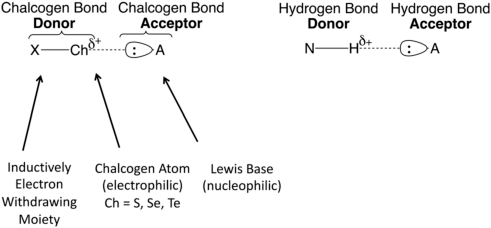
\includegraphics[width=0.8\linewidth]{Figures/ch-bonding.pdf}
    \caption{Chalcogen bonding model, and similarity to H-bonding.}
    \label{fig:ch-bonding}
\end{figure}

The mechanism of chalcogen bonding is believed to involve both electrostatic and orbital interaction components with dispersion being a lesser contributor.
The electrostatic component involves attraction between the Lewis base and a positively charged $\sigma$-hole which is generated along the extension of the \ce{Ch-X} bond due to polarisation of the bonding orbital, while the orbital  interaction component involves mixing between the occupied lone pair orbital of the Lewis base and the vacant $\sigma^{\star}_{\mathrm{Ch-X}}$ bond on the chalcogen, both these interactions account for the directionality of this interaction to different extents. 
Whereas the electrostatic $\sigma$-hole interaction is believed to be the main contributor to the closely related halogen bonding interactions,\autocite{Prasang2009,Sarwar2010,Beale2013,Aakeroy2013,Goud2016,Stone2013} significant lengthening of the \ce{Ch-X} bond observed in the crystal structures of a number of chalcogen bonded systems is suggestive of a significant charge-transfer component to this interaction.\autocite{Fellowes2019,Pascoe2017}

\section{Results and discussion}
As part of our efforts towards a chalcogen-bonding based DNA minor-groove binding agent we required the benzisoselenazolinone \cmpd{ebs-nitroamide-2py}, which we proposed to cyclise to the benzimidazole-substituted  benzisoselenazolinone \cmpd{ebs-rhs-2py}, an analog to the Hoechst-type DNA-binding bisbenzimadazoles.\autocite{Loewe1974,Pjura1987,Martin2004} 

\subsection{Synthesis}
The benzisoselenazolinone \cmpd{ebs-nitroamide-2py} was prepared from the diselenide \cmpd{diselenide} by conversion to the bis-electrophilic selenium reagent \cmpd{dichloride},\autocite{Lesser1924} followed by condensation with 2-nitro-1,4-benzenediamine to give the benzisoselenazolinone \cmpd{ebs-nitroaniline}, which was then coupled to picolinic acid via a Yamaguchi intermediate (\ref{sch:ebs-synthesis2}).

\begin{scheme}
\replacecmpd{diselenide}
\replacecmpd{dichloride}
\replacecmpd{ebs-nitroaniline}
\replacecmpd{ebs-nitroamide-2py}
\replacecmpd{ebs-rhs-2py}
TMP LABELS NOT EMBEDDED AS TEXT. REDO.
%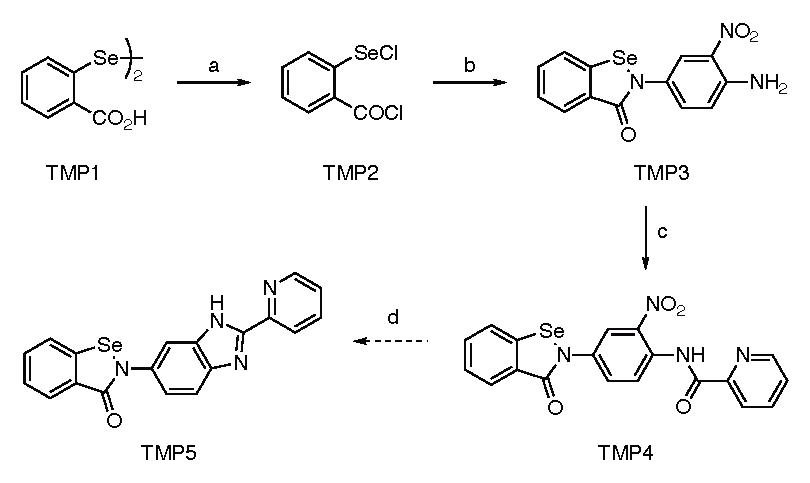
\includegraphics[scale=0.8]{Figures/ebs-synthesis2.eps}
\caption[Synthesis of precursor \refcmpd{ebs-nitroamide-2py}]{Synthesis of precursor \refcmpd{ebs-nitroamide-2py}. a) \ce{SOCl2}, b) 2-nitro-1,4-benzenediamine, \ce{Et3N}, THF, c) Picolinic acid, TCBC/DMAP, \ce{Et3N}, d) [H], \ce{H+}.}
\label{sch:ebs-synthesis2}
\end{scheme}

\subsection{Structural characterisation}
Benzisoselenazoline \cmpd{ebs-nitroamide-2py} was found to be of low solubility in most organic solvents, but very small orange needles were obtained from slow evaporation from dimethylformamide.
The crystal structure obtained using data collected at the Australian Synchrotron was that of a non-solvate form, referred to herein as \cmpd{ebs-nitroamide-2py}(ex.DMF) in the orthorhombic space group Pbca. 
A thermal ellipsoid plot for \cmpd{ebs-nitroamide-2py}(ex.DMF) is presented in \ref{fig:ebs-nitroamide-2py-dmf-xtal}.

\begin{figure}
    \centering
    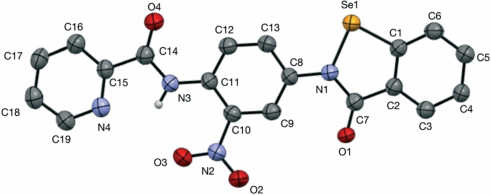
\includegraphics[width=0.8\linewidth]{Figures/ebs-nitroamide-2py-dmf-xtal.pdf}
    \caption{Thermal ellipsoid plot of \refcmpd{ebs-nitroamide-2py}(ex.DMF). Ellipsoids are at the 50\% probability level.}
    \label{fig:ebs-nitroamide-2py-dmf-xtal}
\end{figure}

The crystal packing in \cmpd{ebs-nitroamide-2py}(ex.DMF) is characterised a number of non-covalent interactions including $\pi$-stacking which forms columns extending down the \emph{b} axis between molecules of \cmpd{ebs-nitroamide-2py} related by the \emph{b} glide plane (\ref{fig:ebs-nitroamide-2py-packing}). 
The planes defined by the central aromatic ring C8-C13 are inclined at an angle 10.3(2)\degree to the adjacent $\pi$-stacked molecule, with a centroid (C8-C13) plane distance of 3.414(4)~\AA~and a centroid–centroid distance of 3.786(4)~\AA~representing a slip distance of 1.636~\AA.

\begin{figure}
    \centering
    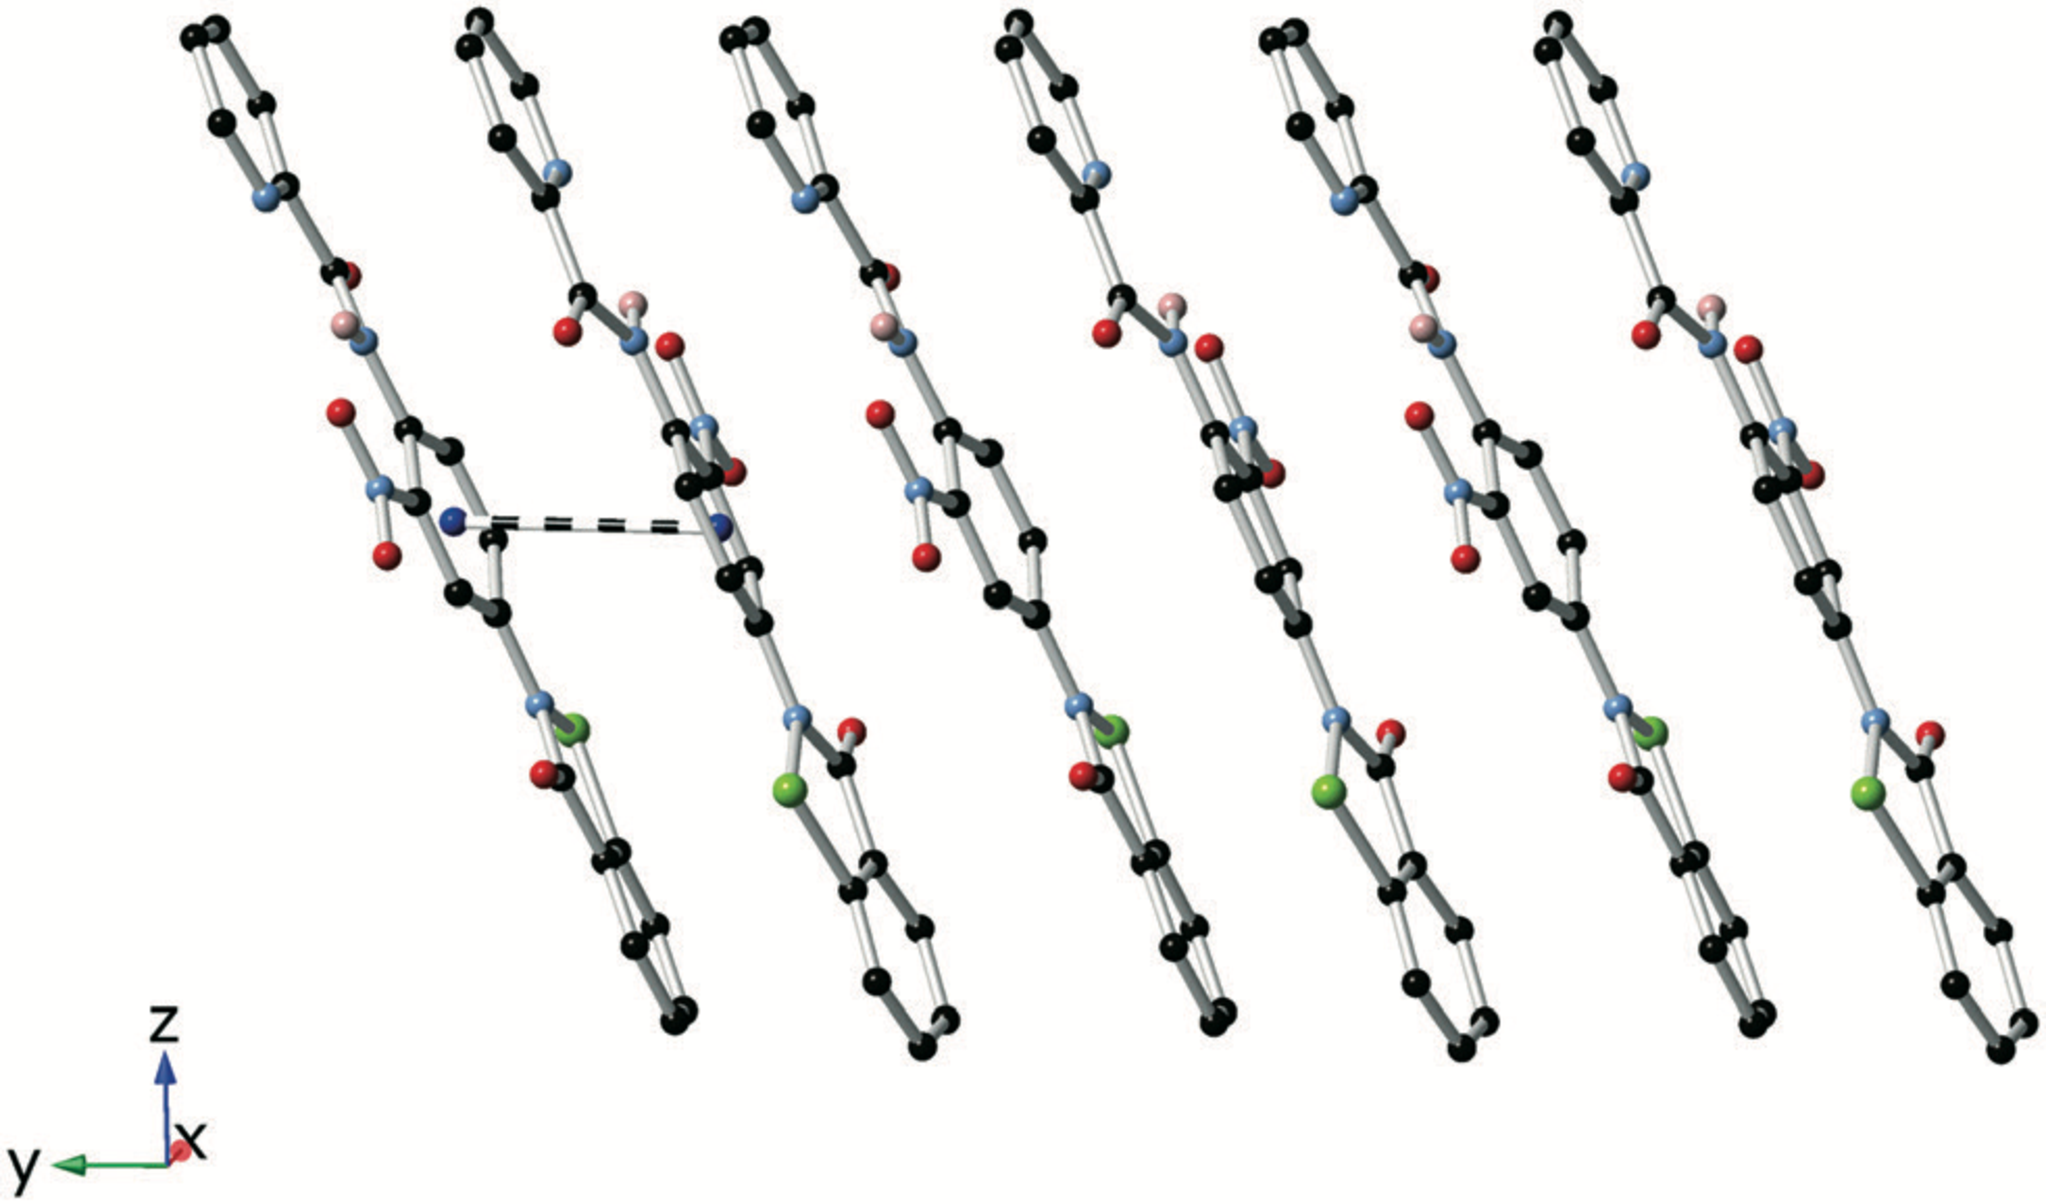
\includegraphics[width=0.8\linewidth]{Figures/ebs-nitroamide-2py-packing.pdf}
    \caption{Offset $\pi$-stacking of \refcmpd{ebs-nitroamide-2py}(ex.DMF) extending down the \emph{b}-axis. The centroid-centroid distance is 3.786(4)~\AA.}
    \label{fig:ebs-nitroamide-2py-packing}
\end{figure}

Adjacent $\pi$-stacked columns are held together by chalcogen bonding interactions between the isoselenazolinone amide carbonyl oxygen and the selenium atom in the heterocyclic ring forming chains generated by the \emph{a}-glide plane extending down the \emph{a}-axis.
The \ce{O\cdots Se} distance is 2.659(3)~\AA~and the \ce{O\cdots Se-N} angle is 173.6(2)\degree.
The angle between the planes defined by the benzisoselenazolinone rings in the chalcogen bonded pairs is 138.8\degree a coplanar arrangement is presumably disfavoured as this would result in severe steric clashes with the C5 of the benzisoselenazolinone ring. 
Similar \ce{O\cdots Se} chalcogen bonding interactions have been observed in other benzisoselenazolinone derivatives related to the drug ebselen with comparable geometries.\autocite{Fellowes2019,Thomas2015,Bhabak2007,Piatek1995} 
The \ce{N{3}-H{3}} group which is flanked by the pyridine nitrogen and the nitro group engages in intramolecular \ce{N-H\cdots N} and \ce{N-H\cdots O} hydrogen bonds, but is not involved in any significant intermolecular interactions (\ref{fig:ebs-nitroamide-2py-o-se}, \ref{fig:ebs-nitroamide-2py-pi-stacking}, \ref{fig:ebs-nitroamide-2py-3d}).

\begin{figure}
    \centering
    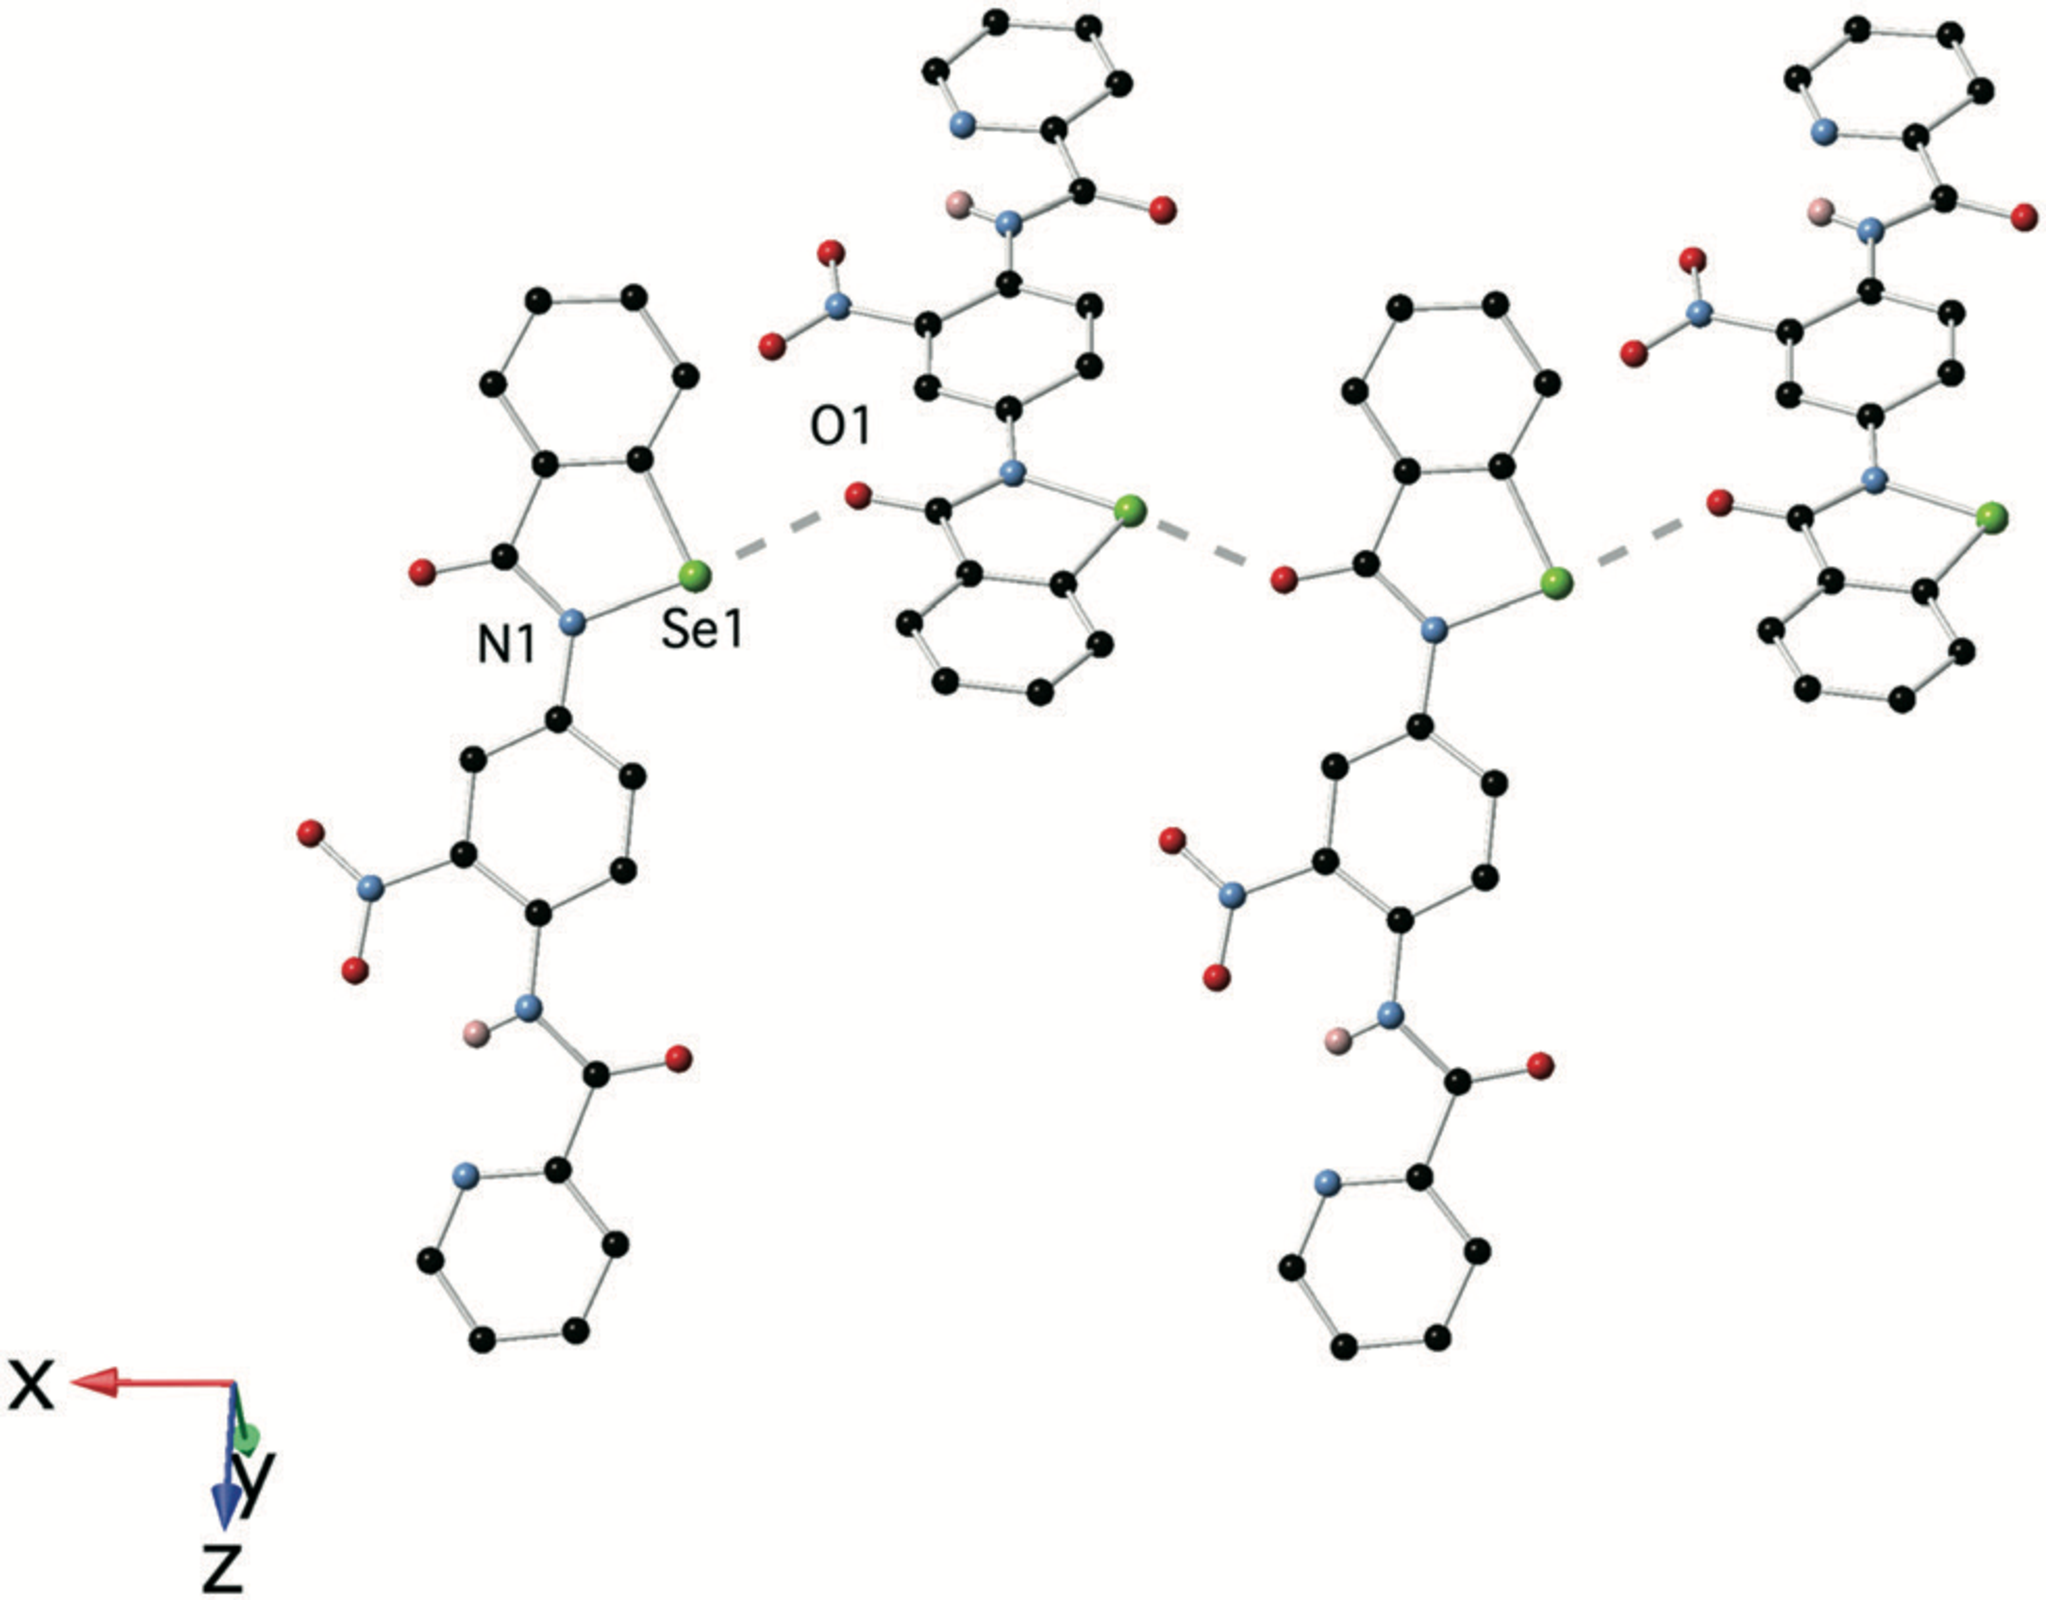
\includegraphics[width=0.8\linewidth]{Figures/ebs-nitroamide-2py-o-se.pdf}
    \caption{\ce{O\cdots Se} chalcogen bonding interactions in \refcmpd{ebs-nitroamide-2py}(ex.DMF).}
    \label{fig:ebs-nitroamide-2py-o-se}
\end{figure}

\begin{figure}
    \centering
    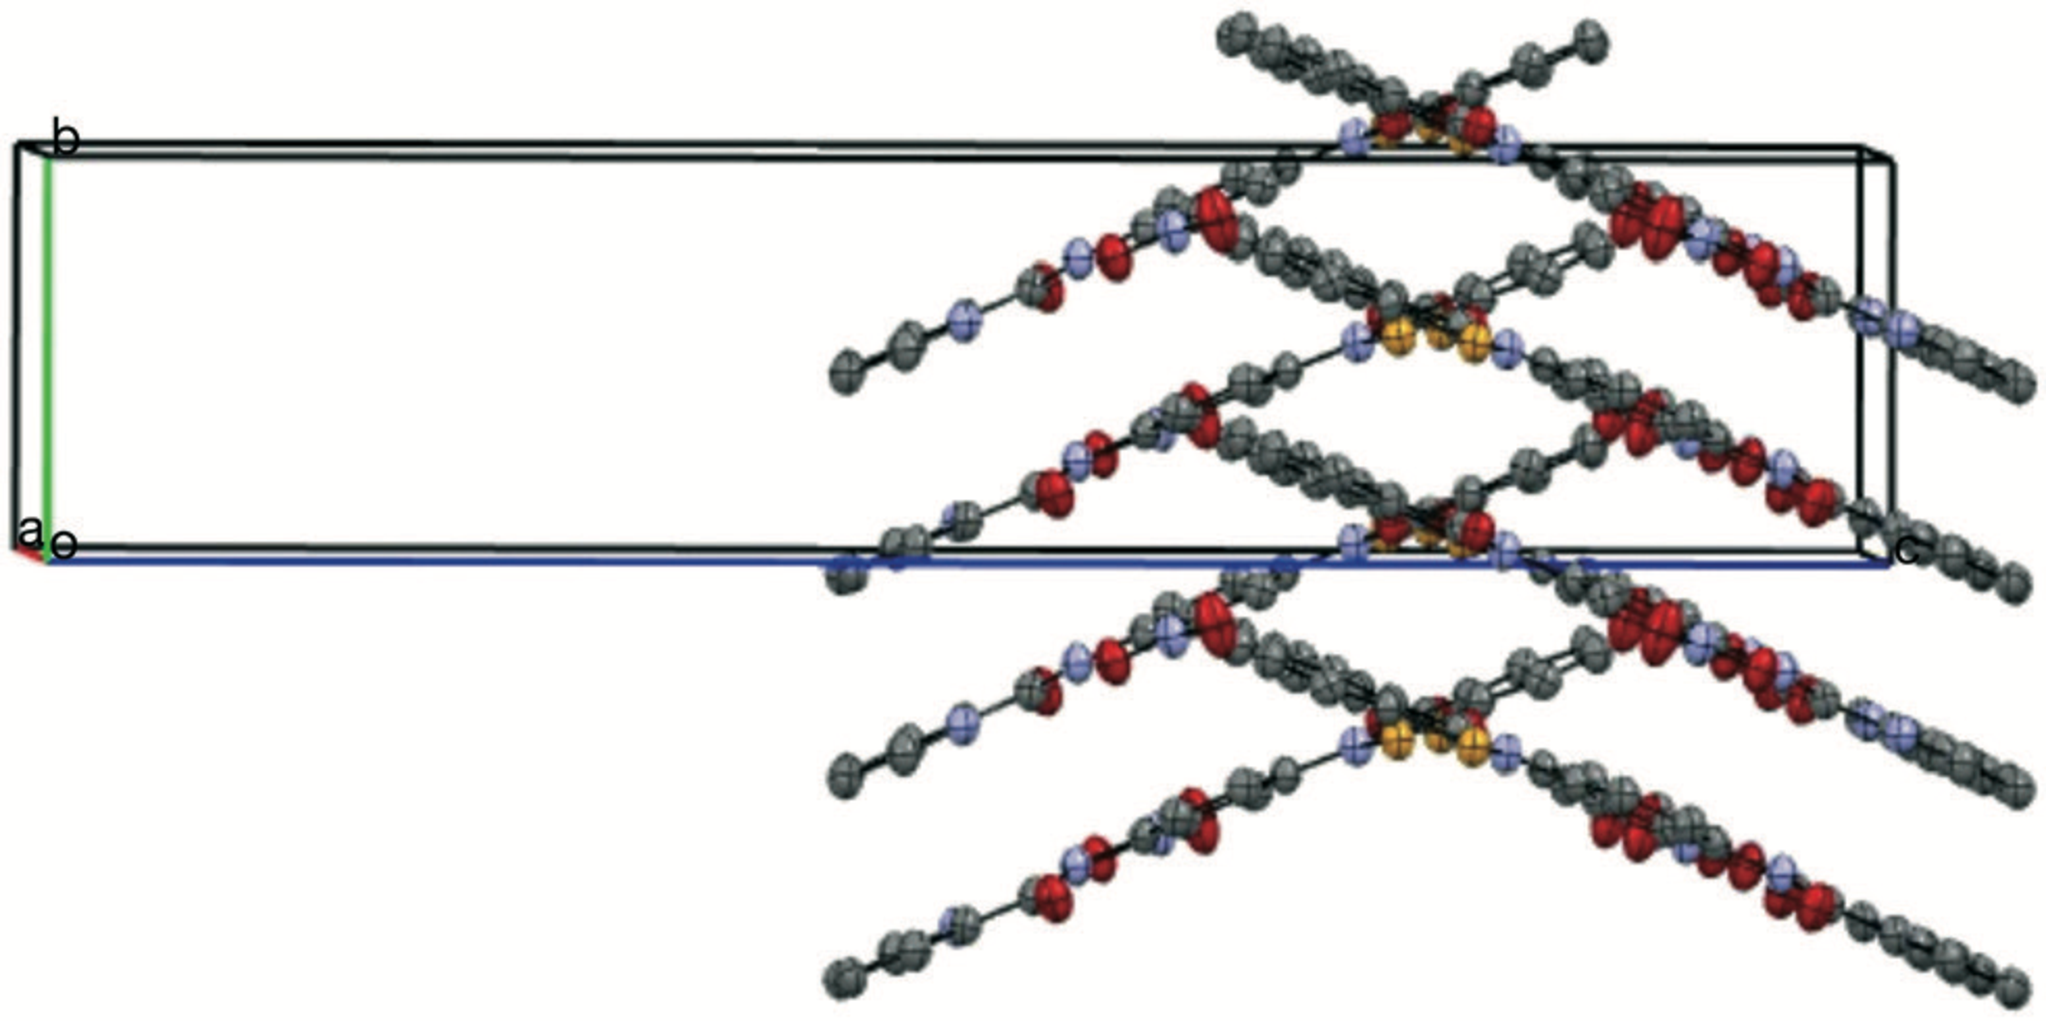
\includegraphics[width=0.8\linewidth]{Figures/ebs-nitroamide-2py-pi-stacking.pdf}
    \caption{2-D layers of \refcmpd{ebs-nitroamide-2py}(ex.DMF) $\pi$-stacking extends along the \emph{b}-axis while the \ce{Se\cdots O} chalcogen bond interactions extend down the \emph{a}-axis.}
    \label{fig:ebs-nitroamide-2py-pi-stacking}
\end{figure}

\begin{figure}
    \centering
    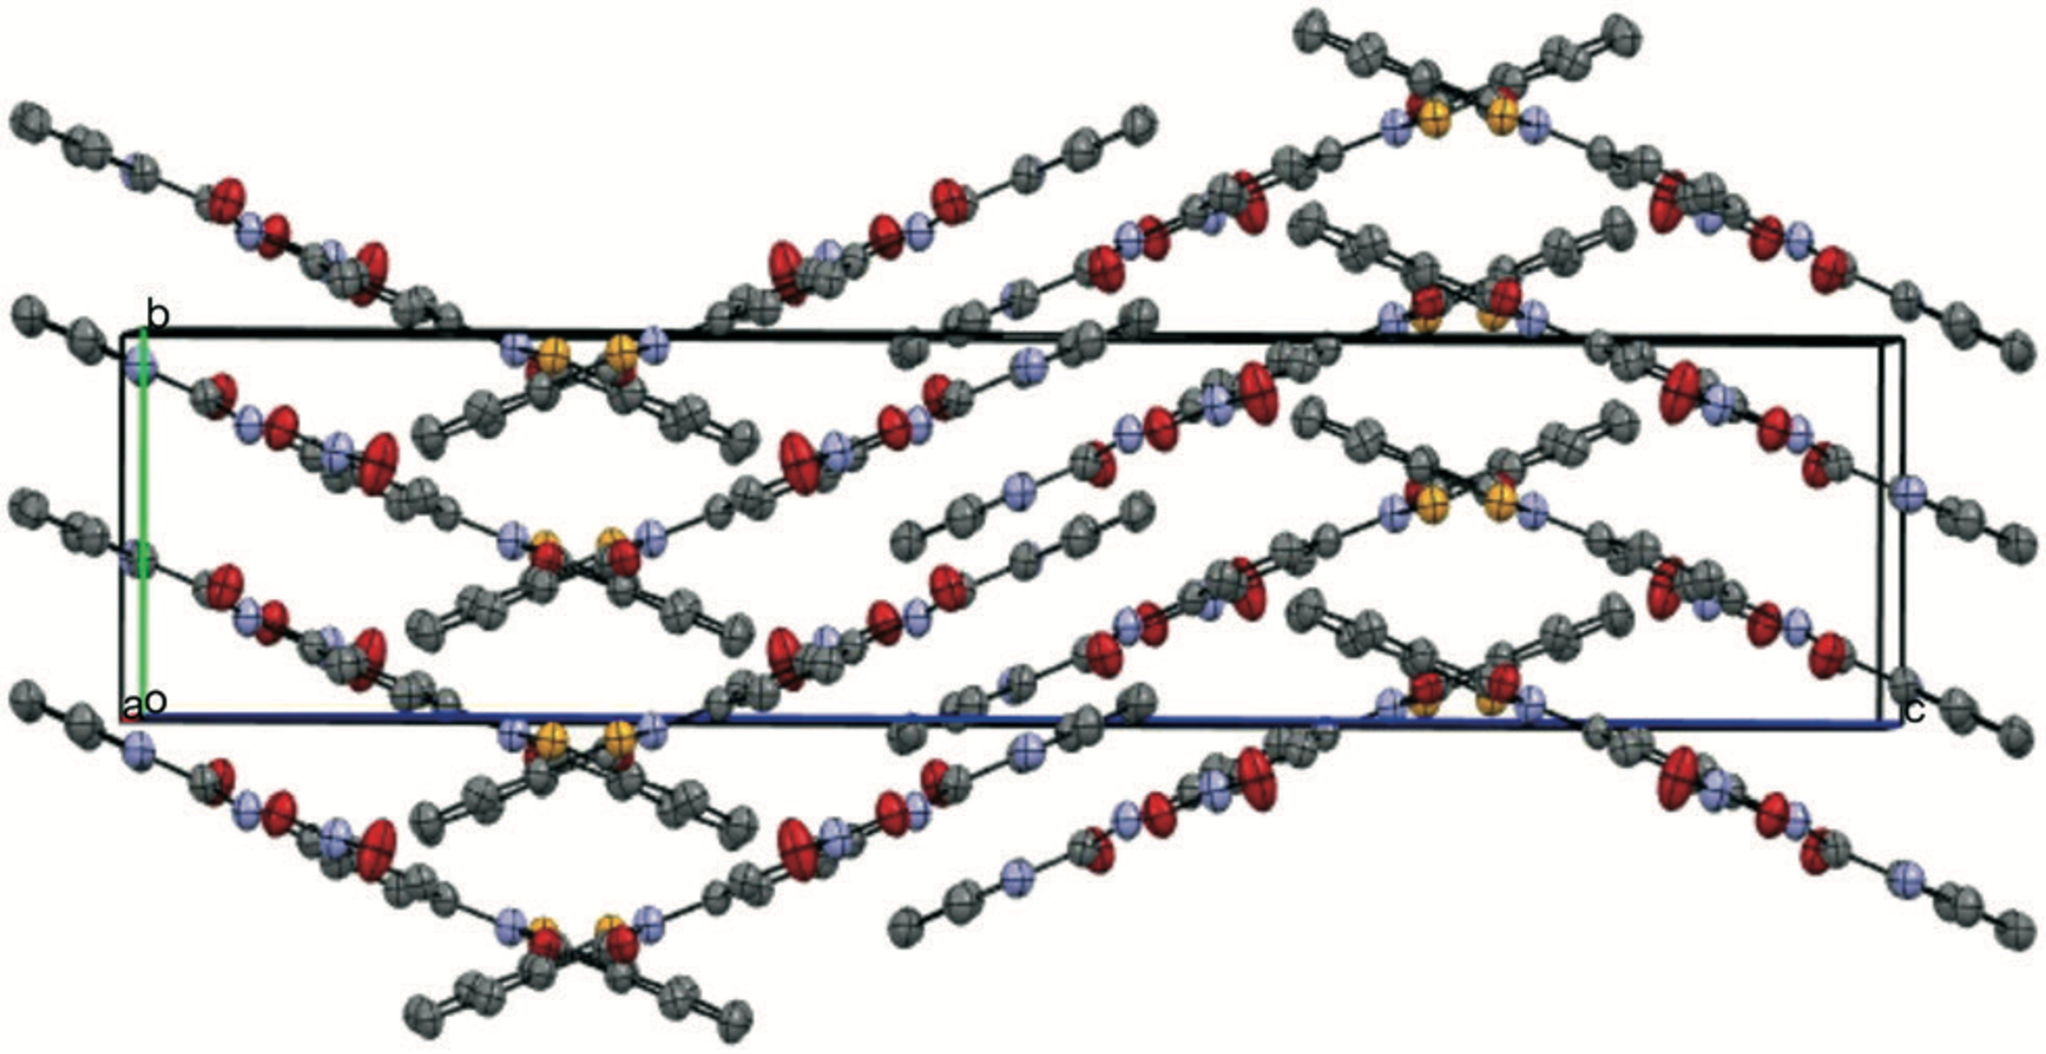
\includegraphics[width=0.8\linewidth]{Figures/ebs-nitroamide-2py-3d.pdf}
    \caption{Extension of the 2-D layers of \refcmpd{ebs-nitroamide-2py}(ex.DMF) into 3-D by van der Waals interactions.}
    \label{fig:ebs-nitroamide-2py-3d}
\end{figure}

The combination of the $\pi$-stacking and chalcogen bonding generates a 2-dimensional network lying parallel to the \emph{ab} plane.
These layers are extended into 3-dimensions by weaker Van-der Waals contacts between molecules related by the \emph{c} glide.

Crystallisation of benzisoselenazolinone \cmpd{ebs-nitroamide-2py} from pyridine gave rise to orange needles which were found to diffract well on the home-source diffractometer. 
The structure solved in the monoclinic space group Pc and was found to be a pyridine solvate, herein labelled \cmpd{ebs-nitroamide-2py}$\cdot$pyridine. 
The structure of \cmpd{ebs-nitroamide-2py}$\cdot$pyridine is presented in \ref{fig:ebs-nitroamide-2py-py-xtal} and shows that the pyridine solvate forms a \ce{N\cdots Se} chalcogen bond between the pyridine solvent molecule and the isoselenazolinone moiety.
The \ce{N{5}\cdots Se{1}} distance is 2.466(5)~\AA, the \ce{N{5}\cdots Se{1}-N{1}} angle is 173.2(2)\degree, and the angle between the plane of the coordinated pyridine ring and the benzisoselenazolinone ring is 89.2(1)\degree.
This geometry compares with previously reported chalcogen bonded adducts involving dimethylaminopyridine with simple benzisoselenazolinones.\autocite{Fellowes2019}
It is interesting to notethat upon formation of the chalcogen bond to pyridine, there is a significant lengthening of the \ce{Se{1}-N{1}} bond distance from 1.910(3)~\AA~in \cmpd{ebs-nitroamide-2py}(ex.DMF) to 1.945(5)~\AA~in \cmpd{ebs-nitroamide-2py}$\cdot$pyridine, which is consistent with the expected structural effects arising from the charge-transfer component of chalcogen-bonding.\autocite{Fellowes2019,Pascoe2017}

\begin{figure}
    \centering
    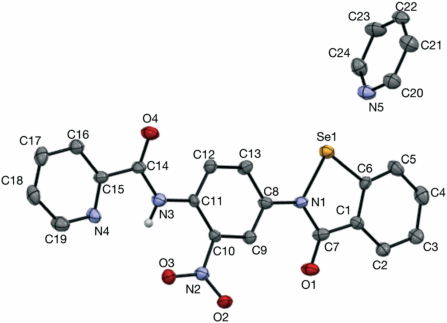
\includegraphics[width=0.8\linewidth]{Figures/ebs-nitroamide-2py-py-xtal.pdf}
    \caption{Thermal ellipsoid plot of \refcmpd{ebs-nitroamide-2py}$\cdot$pyridine. Ellipsoids are at the 50\% probability level.}
    \label{fig:ebs-nitroamide-2py-py-xtal}
\end{figure}

Molecules of \cmpd{ebs-nitroamide-2py} assemble into planar sheets lying parallel to the ($\bar{1} 0 4$) plane, the distance between these sheets as defined by the distance between the centroid of the atoms \ce{C{8}-C{13}} and the adjacent plane is 3.336~\AA~while the centroid-centroid distance is 4.973~\AA~representing a slippage of 3.688~\AA~(\ref{fig:ebs-nitroamide-2py-sheets-1}, \ref{fig:ebs-nitroamide-2py-sheets-2}).
The parallel sheets of molecules of \cmpd{ebs-nitroamide-2py} are pierced by channels of chalcogen bonded pyridine molecules which run parallel to the \emph{a}-axis at an angle of approximately 133\degree~to the plane.

\begin{figure}
    \centering
    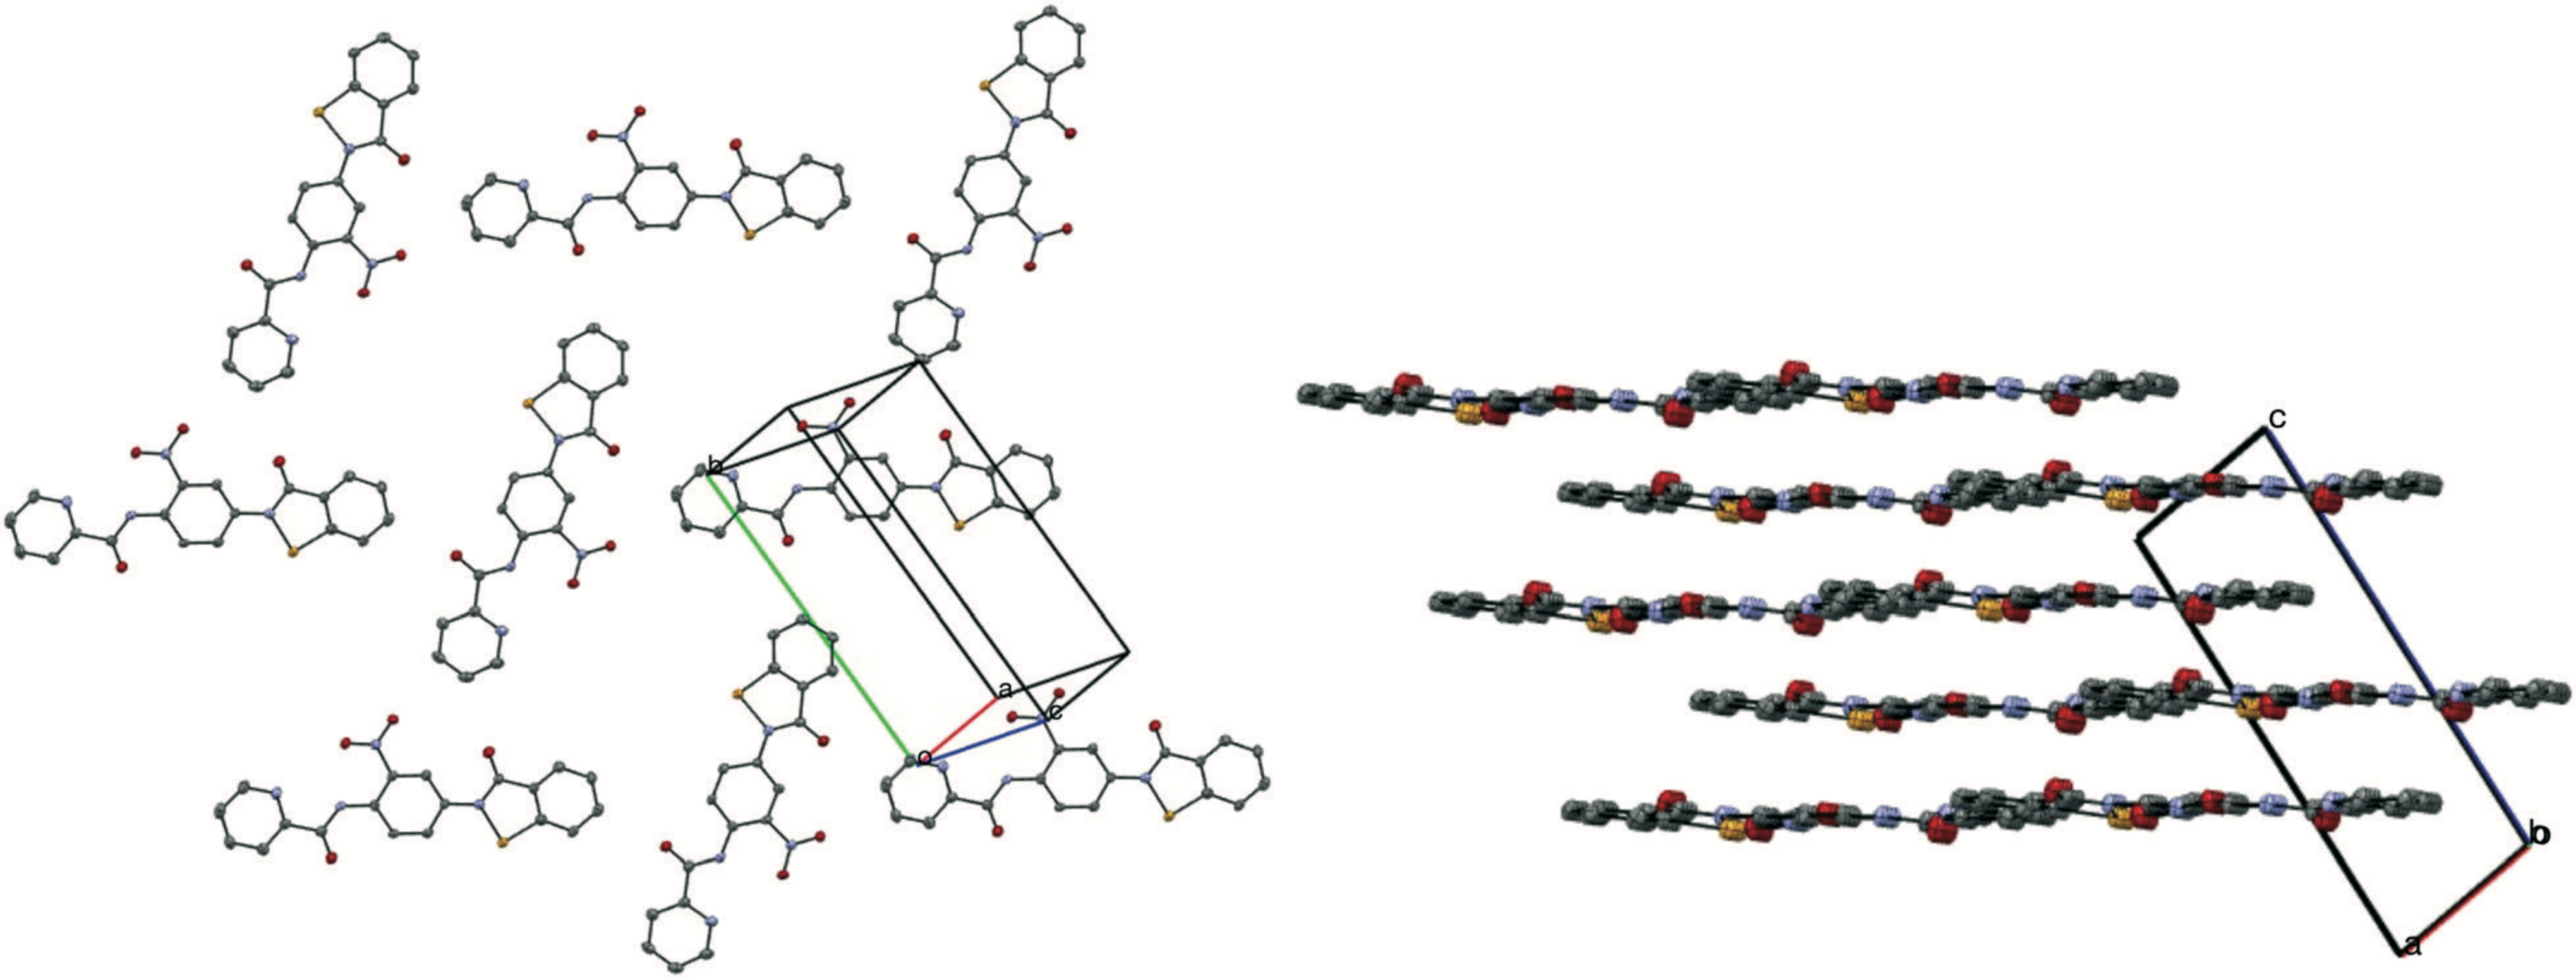
\includegraphics[width=0.8\linewidth]{Figures/ebs-nitroamide-2py-sheets-1.pdf}
    \caption{Sheets of compound \refcmpd{ebs-nitroamide-2py} viewed from orthogonal and parallel directions. Pyridine solvate has been excluded.}
    \label{fig:ebs-nitroamide-2py-sheets-1}
\end{figure}

\begin{figure}
    \centering
    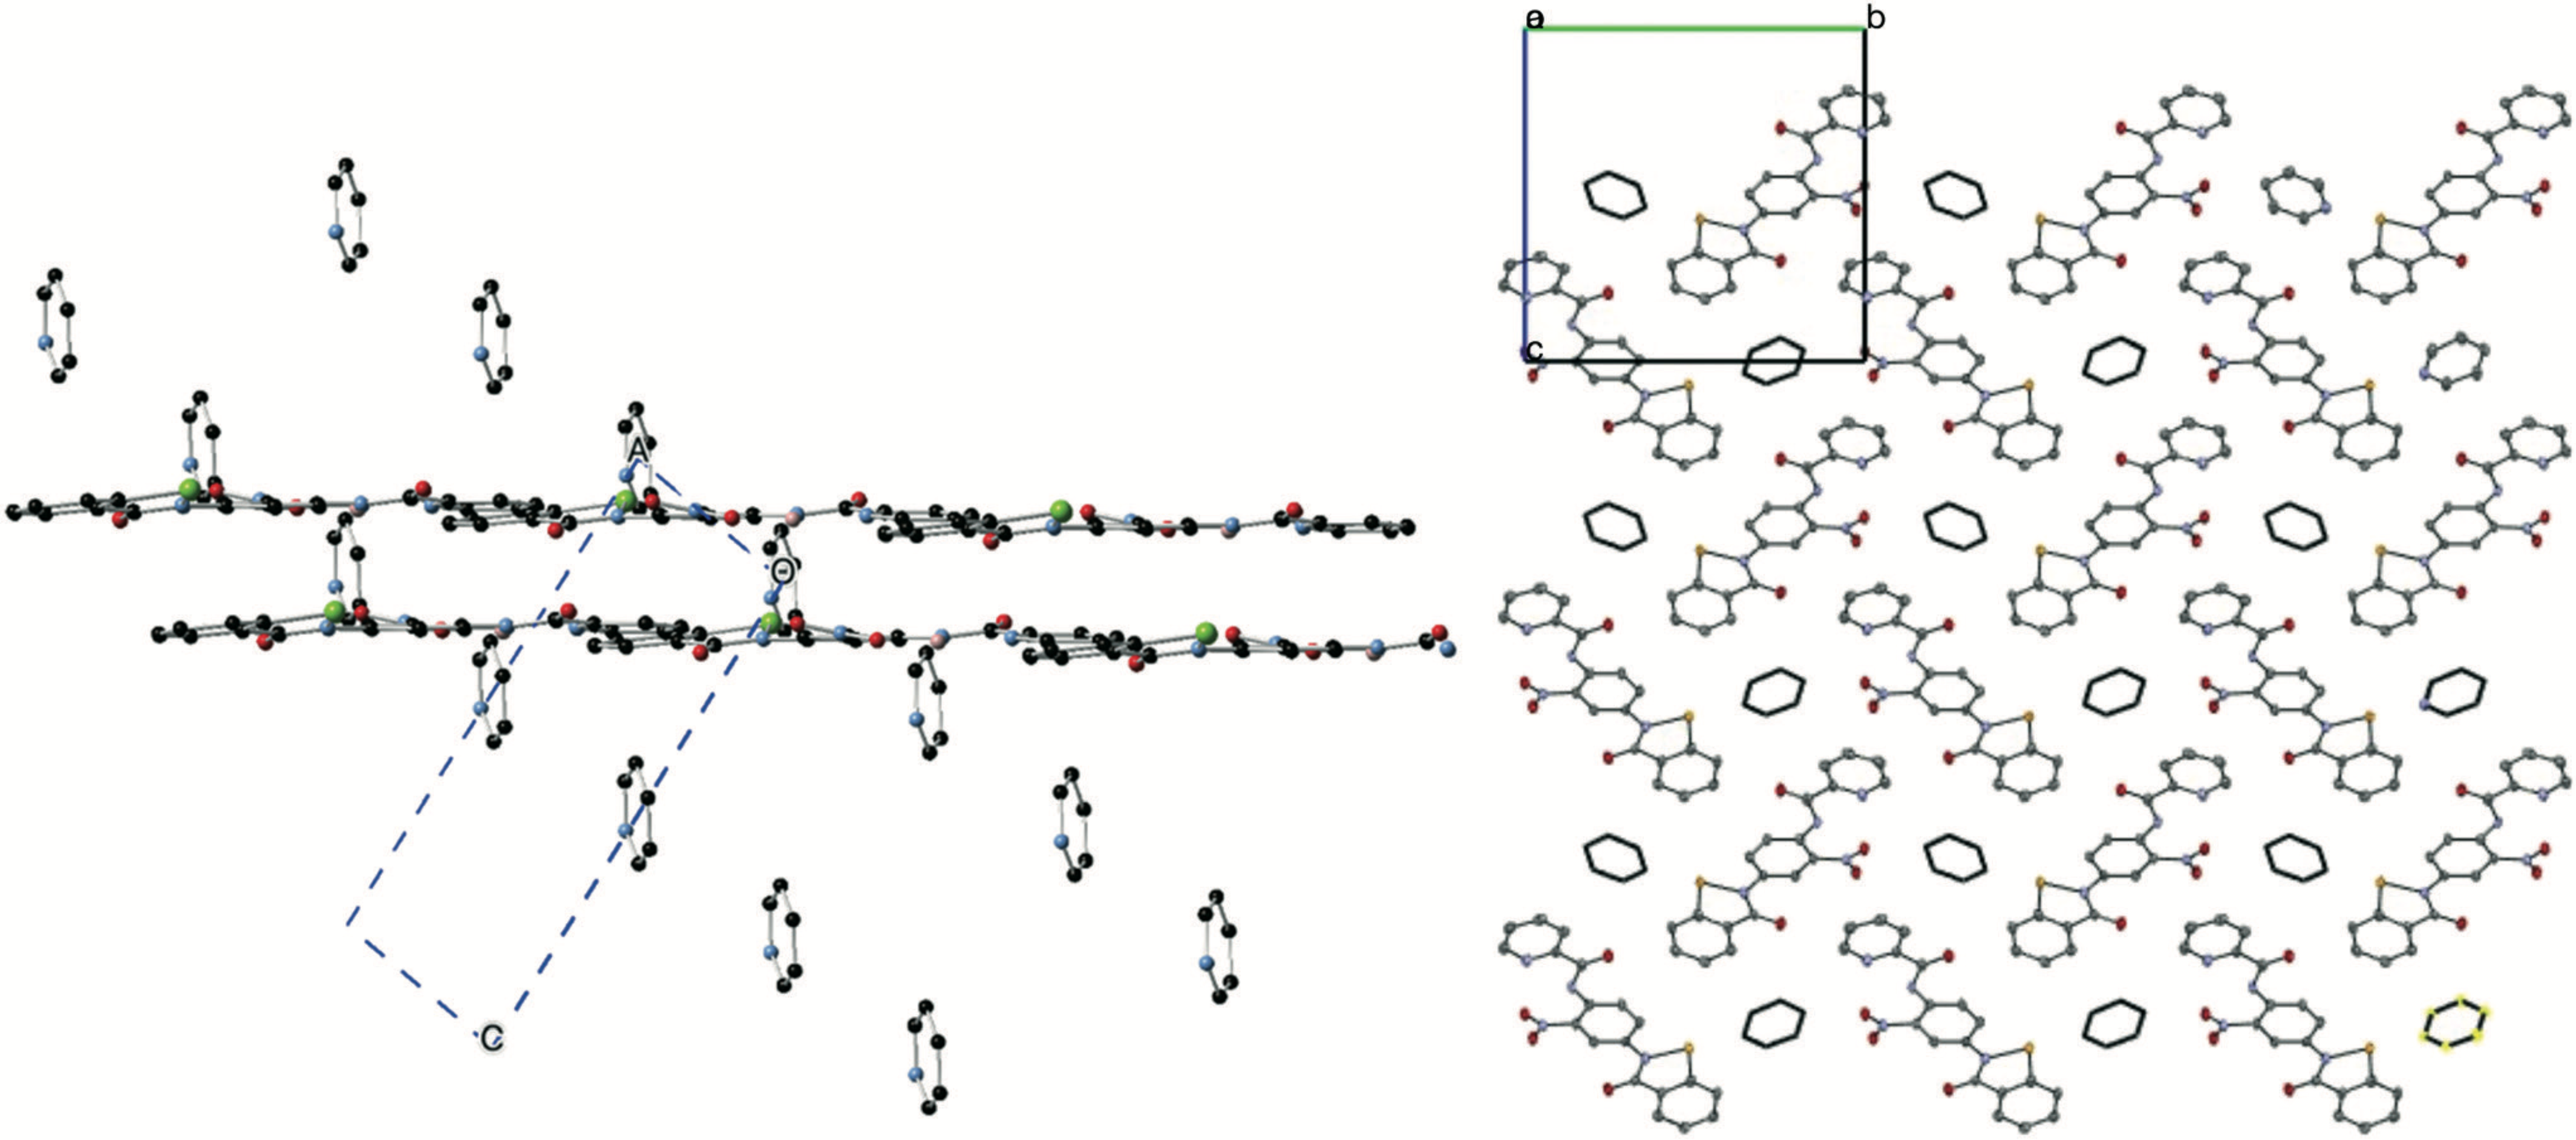
\includegraphics[width=0.8\linewidth]{Figures/ebs-nitroamide-2py-sheets-2.pdf}
    \caption{Two orthogonal views of parallel sheets of compound \refcmpd{ebs-nitroamide-2py}, pierced by channels of pyridine molecules running parallel to the \emph{a}-axis.}
    \label{fig:ebs-nitroamide-2py-sheets-2}
\end{figure}

\subsection{Variable temperature studies}
Thermal gravimetric analysis of the pyridine solvate \cmpd{ebs-nitroamide-2py}$\cdot$pyridine was conducted on a Mettler TGA/SDTA851 apparatus in 40~$\mu$L aluminium crucibles. 
A mass loss of 15.04\% occurred between 90--110\degree C corresponding to the loss of the pyridine solvate (calc. 15.26\%) followed by a second loss of 24.73\% between 300--360\degree C which is consistent with the loss of 121 a.m.u. very likely associated with the Pyr-C(O)NH moiety (\ref{fig:tga}).

\begin{figure}
    \centering
    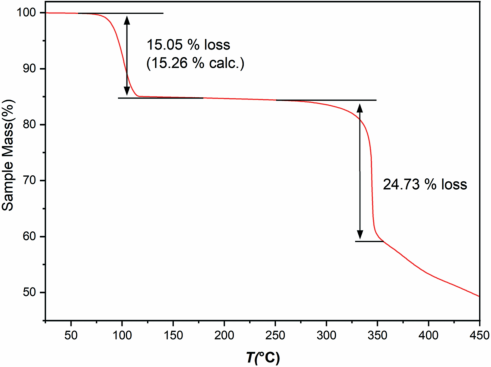
\includegraphics[width=0.8\linewidth]{Figures/tga.pdf}
    \caption{TGA analysis of \refcmpd{ebs-nitroamide-2py}$\cdot$pyridine}
    \label{fig:tga}
\end{figure}

The observation that both the non-solvate \cmpd{ebs-nitroamide-2py}(ex.DMF) and \cmpd{ebs-nitroamide-2py}$\cdot$pyridine had the same melting point (experimental section below) intrigued us to establish whether desolvation of \cmpd{ebs-nitroamide-2py}$\cdot$pyridine which occurs between 90--120\degree C results in conversion to non-solvate \cmpd{ebs-nitroamide-2py}(ex.DMF). 
Thus we carried out variable temperature powder X-ray diffraction measurements on \cmpd{ebs-nitroamide-2py}$\cdot$pyridine from -173\degree C to 117\degree C.
The resulting diffractograms are shown in \ref{fig:vt-pdx}.

\begin{figure}
    \centering
    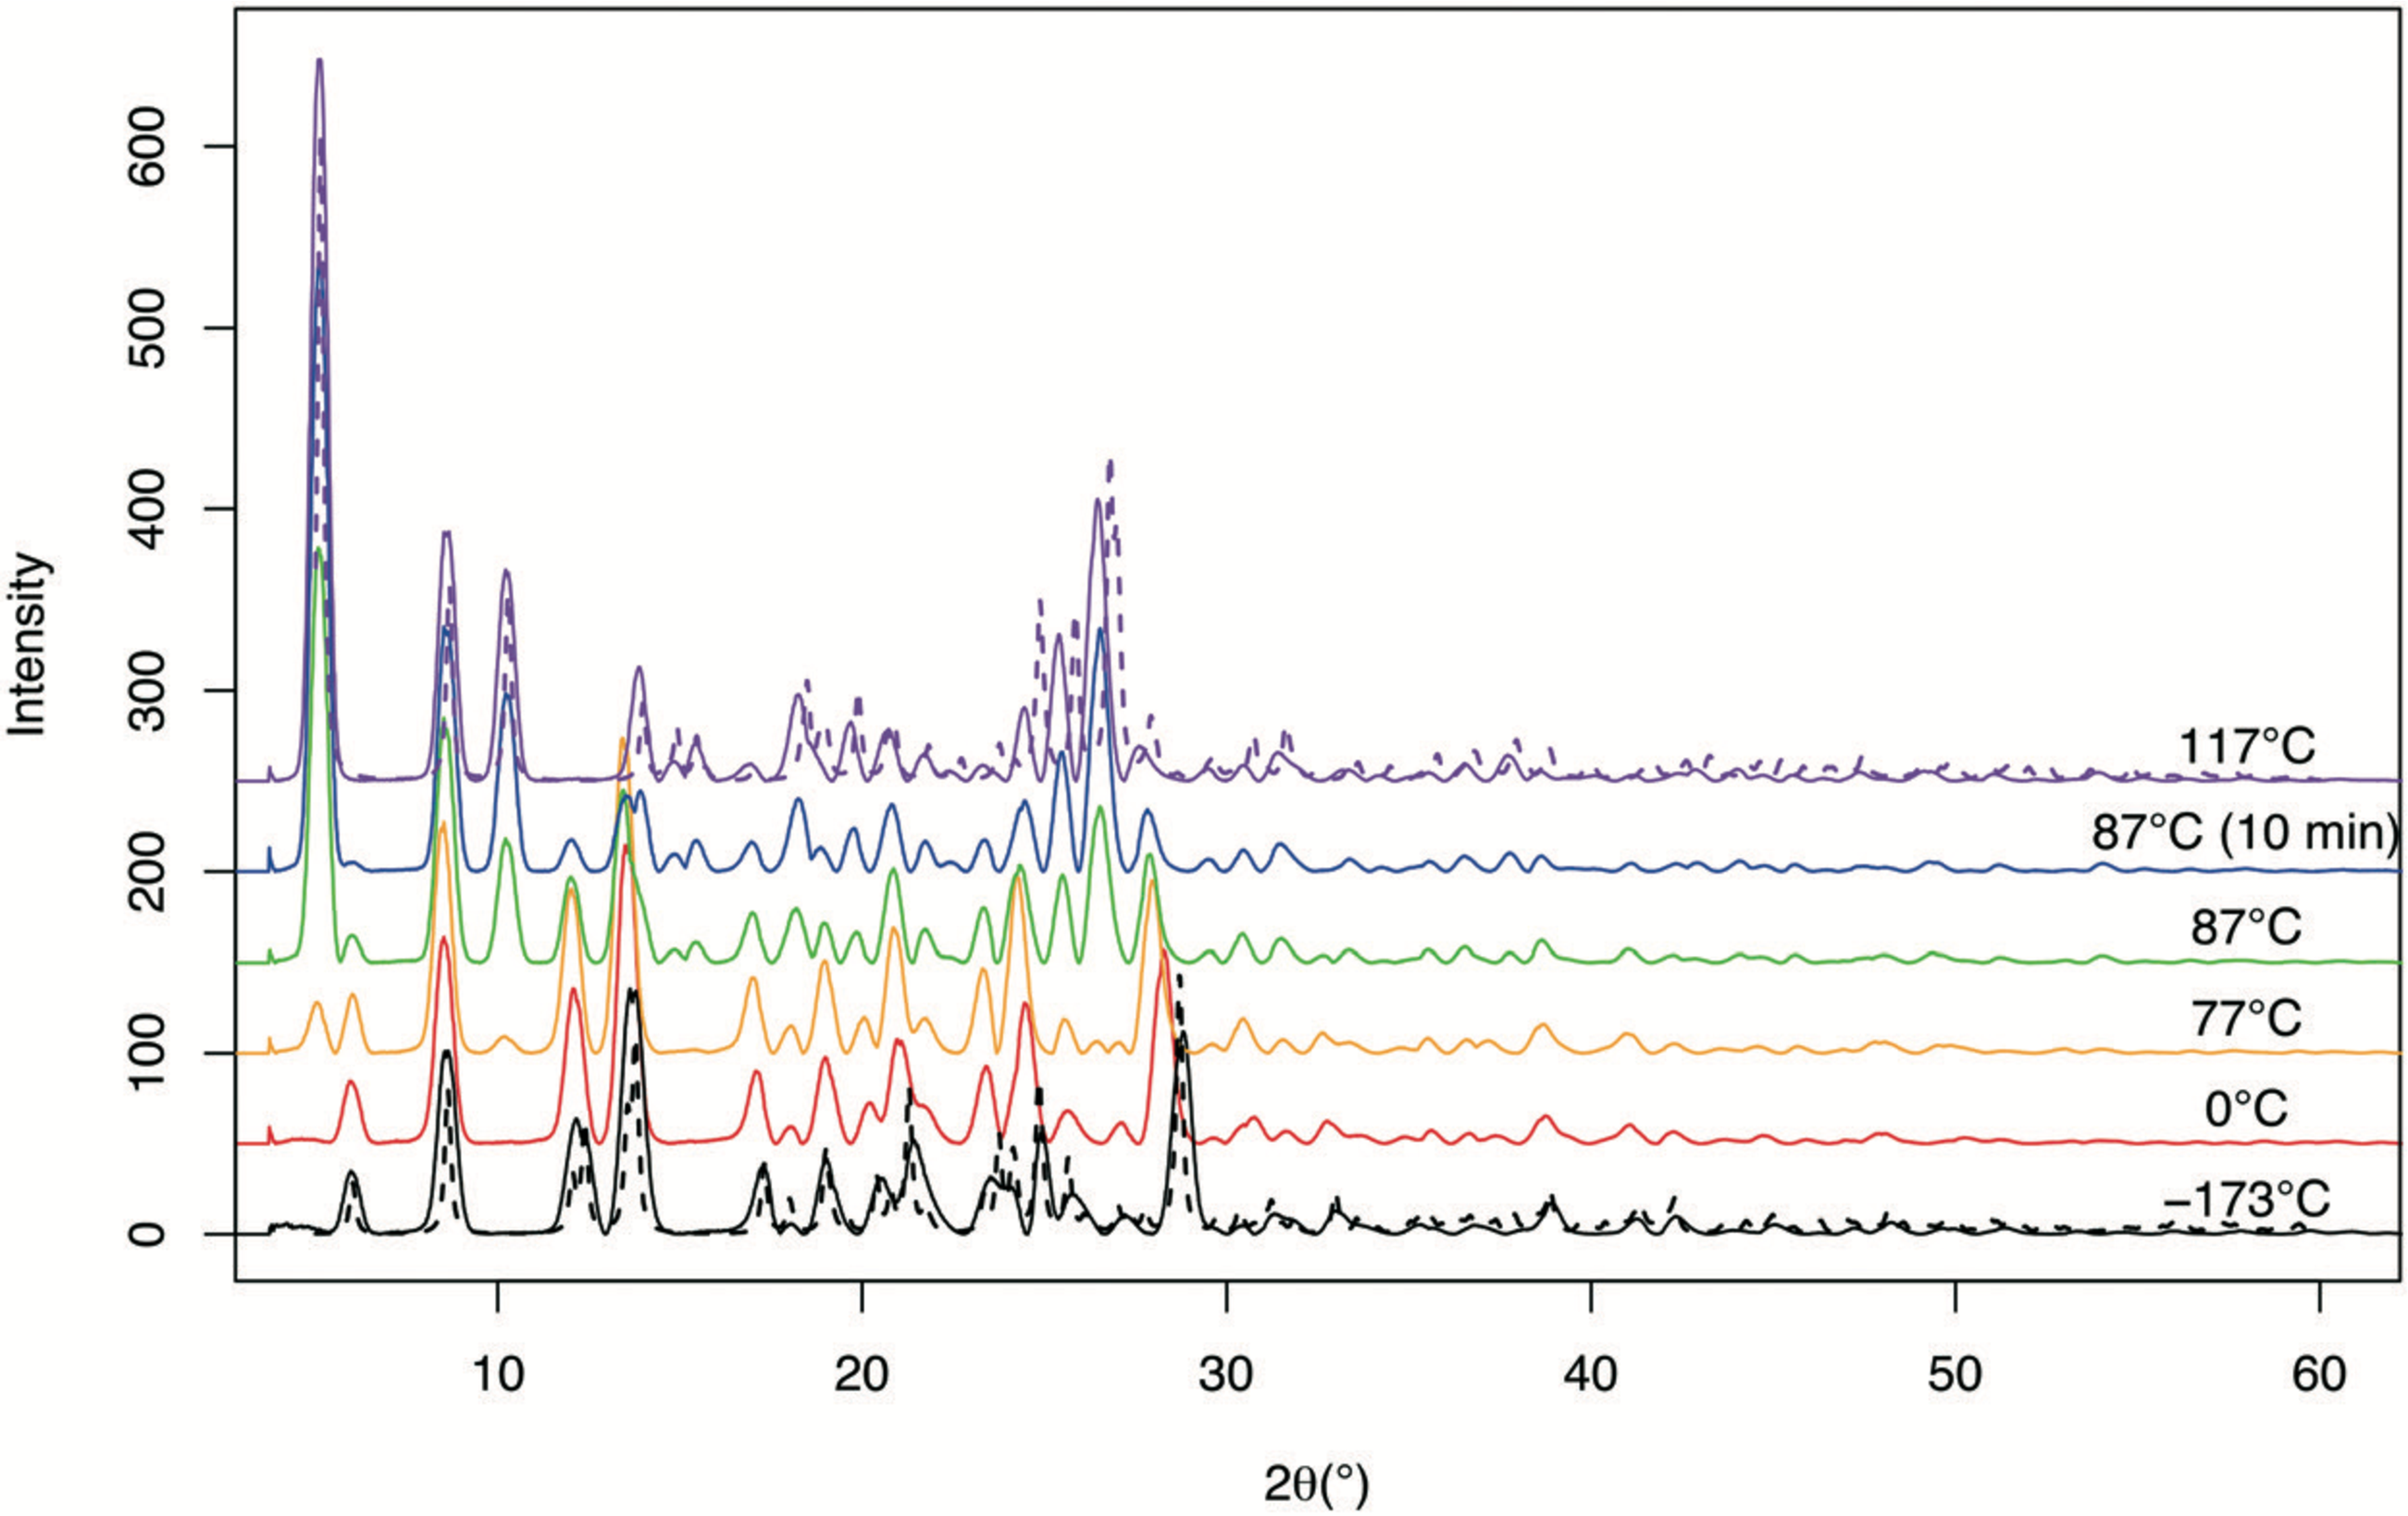
\includegraphics[width=\linewidth]{Figures/vt-pdx.pdf}
    \caption[Variable temperature powder XRD patterns from \refcmpd{ebs-nitroamide-2py}$\cdot$pyridine]{Variable temperature powder XRD patterns from \refcmpd{ebs-nitroamide-2py}$\cdot$pyridine, calculated powder pattern for \refcmpd{ebs-nitroamide-2py}$\cdot$pyridine and \refcmpd{ebs-nitroamide-2py}(ex.DMF) are the dotted lines in the top and bottom traces respectively.}
    \label{fig:vt-pdx}
\end{figure}

From 87\degree C to 117\degree C when pyridine is known to be lost from the sample from the TGA analysis, there is a smooth change from one crystalline phase to another.
Furthermore comparison of the final diffractogram obtained after being kept at 117\degree C for 10 minutes very closely matches the calculated powder pattern for the non-solvate \cmpd{ebs-nitroamide-2py}(ex.DMF) suggesting the transformation from \cmpd{ebs-nitroamide-2py}$\cdot$pyridine into \cmpd{ebs-nitroamide-2py}(ex.DMF).
The same experiment was applied to a single crystal of \cmpd{ebs-nitroamide-2py}$\cdot$pyridine glued on a glass fibre to establish whether this transformation occurs from a single crystal of \cmpd{ebs-nitroamide-2py}$\cdot$pyridine to a single crystal of \cmpd{ebs-nitroamide-2py}(ex.DMF). 
The crystal was heated to 90\degree C and heated at a rate of 0.5\degree C per minute to 120\degree C.
While there was a steady decrease in the intensity of the reflections for \cmpd{ebs-nitroamide-2py}$\cdot$pyridine, individual reflections consistent with a single crystal of \cmpd{ebs-nitroamide-2py}(ex.DMF) were not observed, but rather, there was the development of the powder pattern for \cmpd{ebs-nitroamide-2py}(ex.DMF). 
Interestingly, throughout this transformation the crystal morphology did not appear to change significantly, but the final diffraction pattern was clearly that of a powder.
It is likely that the transformation (which must begin at the surface of the crystal) results in fragmentation of daughter crystals of the non-solvate, thus eroding away at the mother crystal.
We believe that a single crystal to single crystal transformation is very unlikely as collapsing of the channels containing the pyridine solvate would prevent complete desolvation. 
A plausible mechanism for this interconversion likely involves replacement of the \ce{N\cdots Se} chalcogen bond in \cmpd{ebs-nitroamide-2py}$\cdot$pyridine, with a \ce{O\cdots Se} chalcogen bond involving the isoselenazolinone carbonyl group from a molecule in an adjacent layer which is at a distance of 12.051~\AA~(\ref{fig:ebs-nitroamide-2py-transformation}).

\begin{figure}
    \centering
    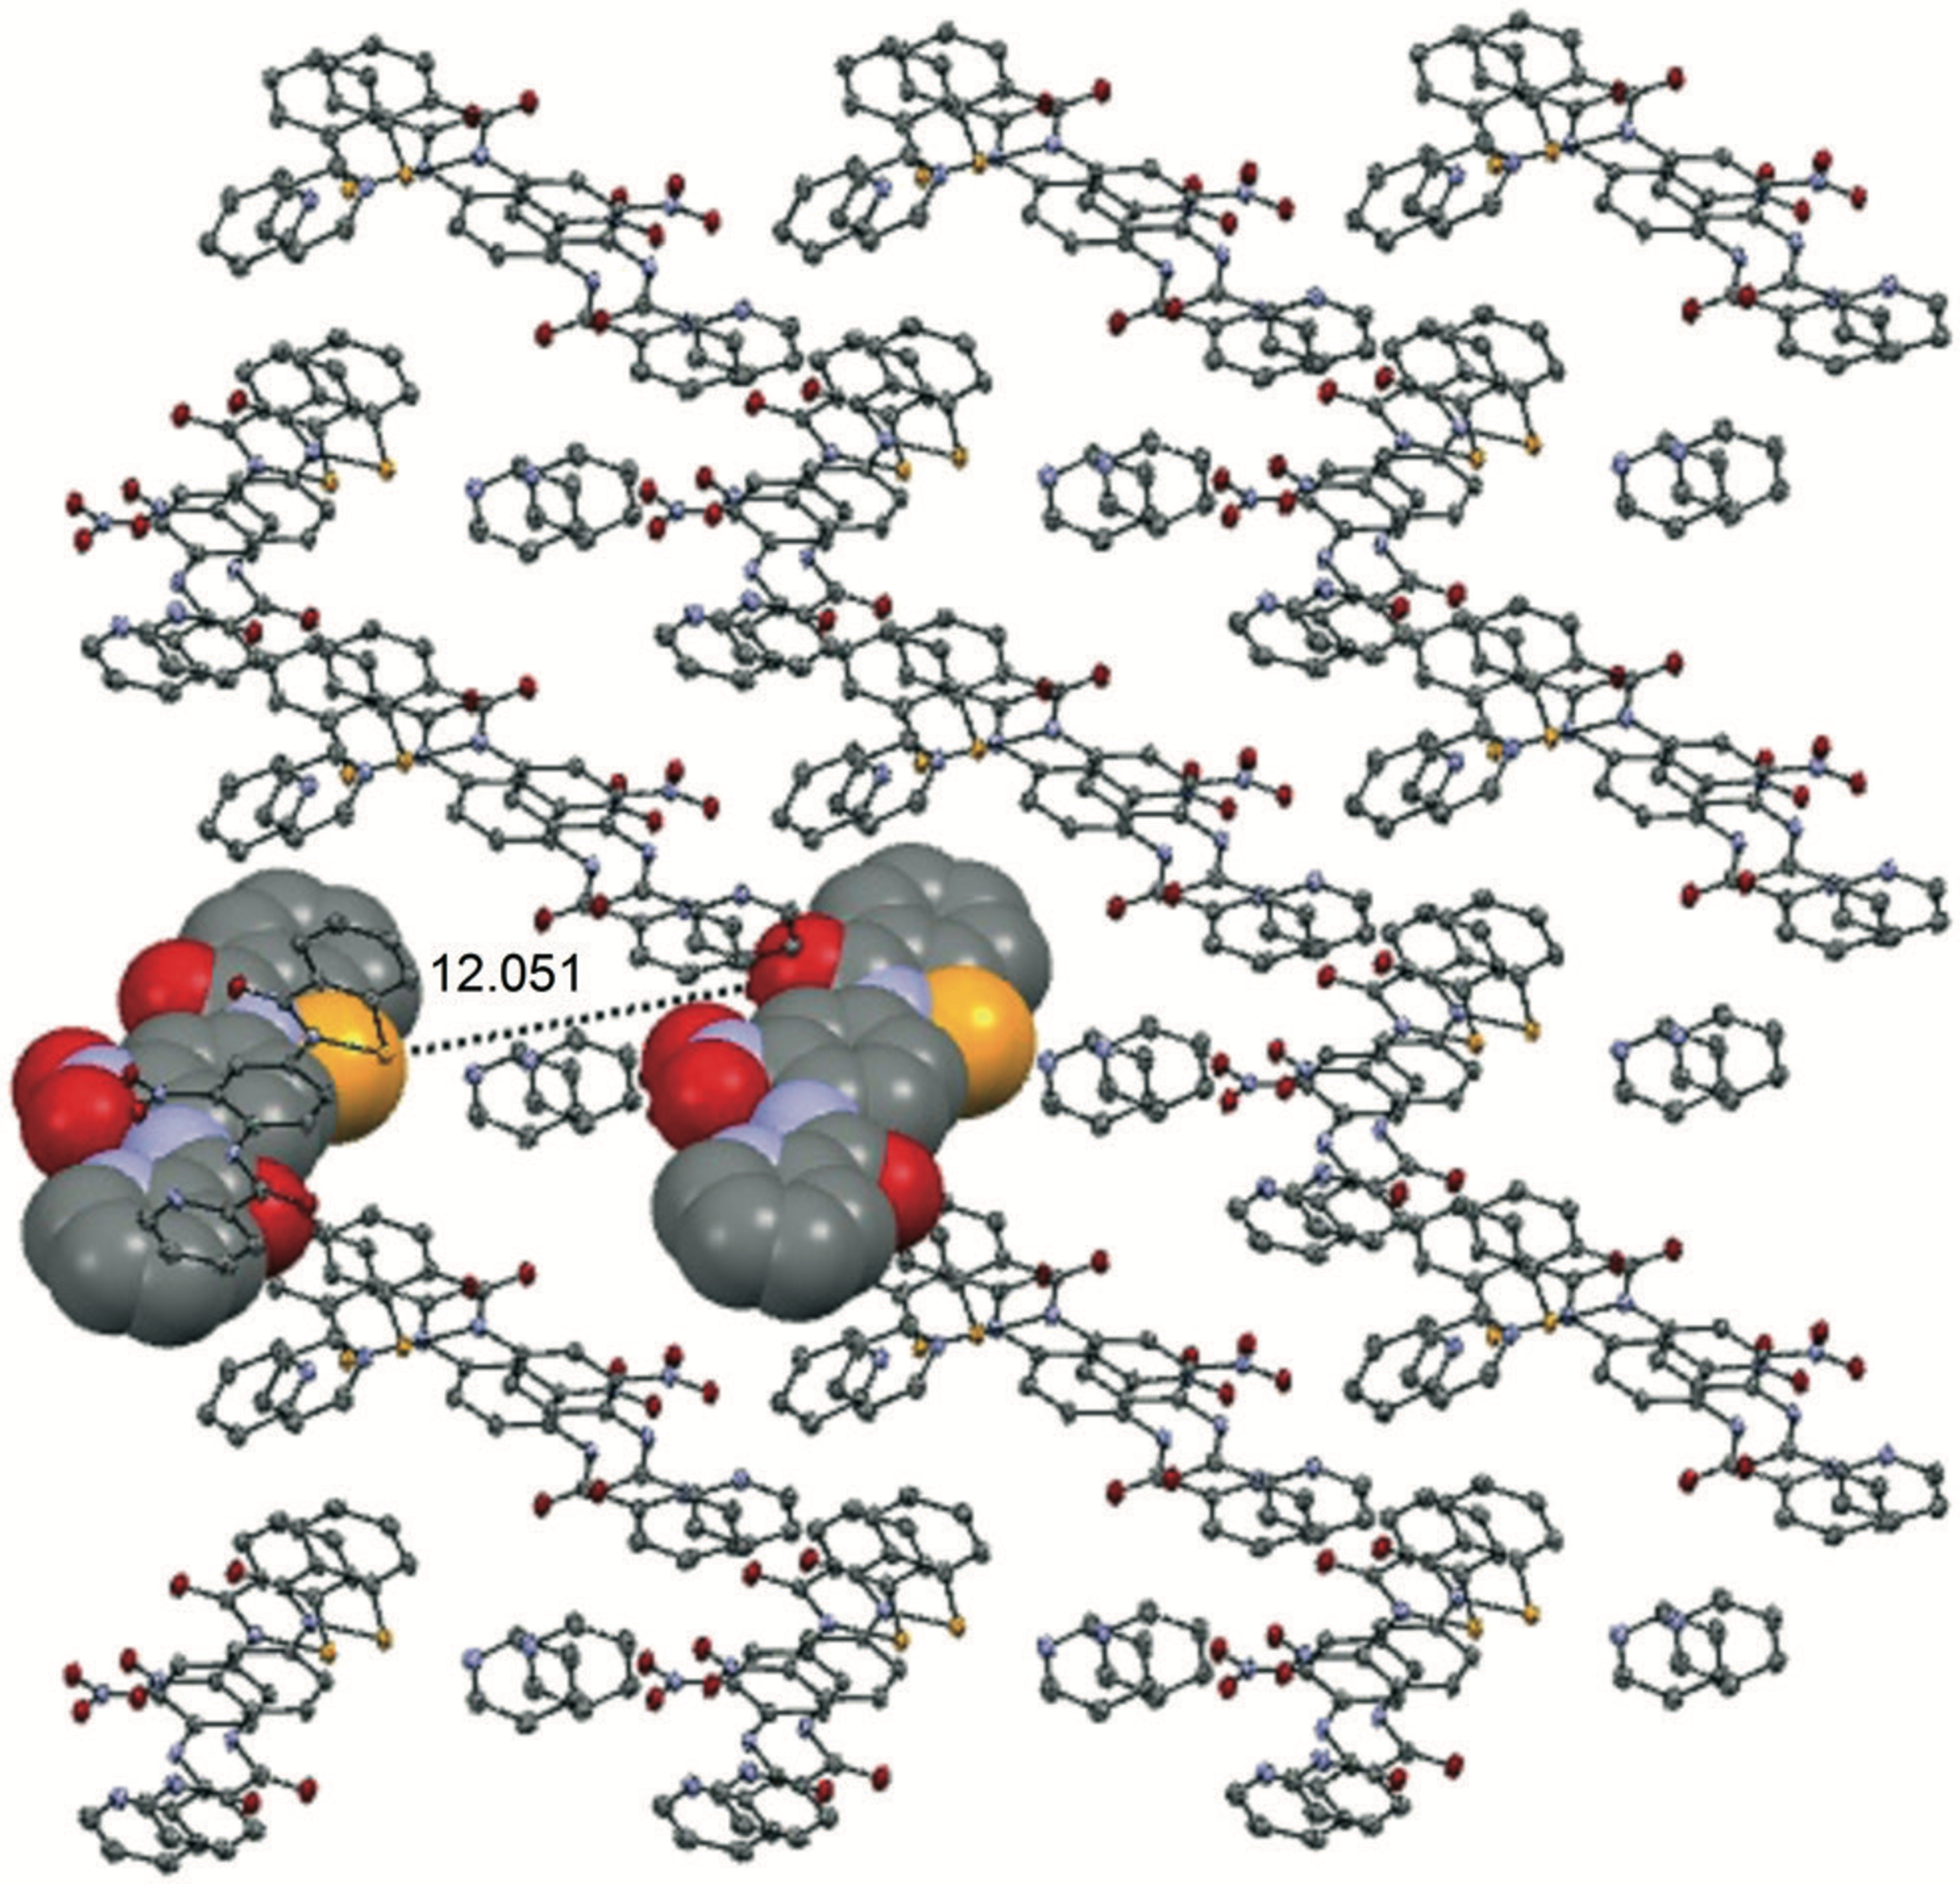
\includegraphics[width=0.8\linewidth]{Figures/ebs-nitroamide-2py-transformation.pdf}
    \caption{Interlayer benzisoselenazolinones \refcmpd{ebs-nitroamide-2py} believed to form a \ce{O\cdots Se} chalcogen bond upon desolvation of \refcmpd{ebs-nitroamide-2py}$\cdot$pyridine.}
    \label{fig:ebs-nitroamide-2py-transformation}
\end{figure}

\section{Conclusion}
The structure of \cmpd{ebs-nitroamide-2py}$\cdot$pyridine is characterised by planar sheets of the benzisoselenazolinone \cmpd{ebs-nitroamide-2py} pierced by channels of pyridine molecules at an angle 133\degree, the pyridine molecules are held in place by \ce{N\cdots Se} chalcogen bonding to the isoselenazolinone moiety.
These channels which extend throughthe structure to the surface of the crystal provide a means for escape of pyridine from the lattice when the crystal is heated to ca. 100\degree C.
Upon loss of the pyridine from these channels the remaining molecules undergo rearrangement to fill the space and in doing so the \ce{N\cdots Se} chalcogen bond in \cmpd{ebs-nitroamide-2py}$\cdot$pyridine is replaced by a \ce{C=O\cdots Se} chalcogen bond to give the non solvate \cmpd{ebs-nitroamide-2py}(ex.DMF). 
The geometry of the chalcogen bond requires that the two benzisoselenazolinone ring systems which are essentially coplanar in \cmpd{ebs-nitroamide-2py}$\cdot$pyridine twist by an angle of 138\degree~resulting in the formation of highly corrugated sheets in the non solvate.

\section{Experimental}
\subsection{Synthesis}
\subsubsection[Preparation of \refcmpd{ebs-nitroaniline}]{Preparation of 2-(4-amino-3-nitrophenyl)benzo[\emph{d}][1,2]-selenazol-3(2\emph{H})-one \refcmpd{ebs-nitroaniline}.}

Diselenide \cmpd{diselenide} (1.2025~g, 3.005~mmol) was dissolved in thionyl chloride (20~mL) and refluxed for 30~min, and the colour changed from purple to light yellow. 
Excess thionyl chloride was removed \emph{in vacuo}, and the residue dissolved in anhydrous THF (50~mL). 
To this was added a solution of 2-nitro-1,4-phenylenediamine (991.9~mg, 6.477~mmol) and triethylamine (dist. from \ce{CaH2}, 3~mL) in anhydrous THF (50~mL). 
This mixture was stirred at room temperature for 18~h, then filtered, washing the precipitate with water, to afford 2-(4-amino-3-nitro-phenyl)benzo[\emph{d}][1,2]-selenazol-3(2\emph{H})-one \cmpd{ebs-nitroaniline} as a brick red solid (940~mg, 61\%, m.p. 300.8--302.0\degree C (DMF)).

{\footnotesize

\ce{^{1}H} NMR (400~MHz, \ce{\emph{d}6}-DMSO) $\delta$ ppm
7.08 (d, \emph{J} = 9.00~Hz, 1~H), 7.46 (t, \emph{J} = 7.43~Hz, 1~H), 7.55 (s, 2~H), 7.59--7.70 (m, 2~H), 7.86 (d, \emph{J} = 7.43~Hz, 1~H), 8.06 (d, \emph{J} = 7.83~Hz, 1~H), 8.12 (d, \emph{J} = 1.96~Hz, 1~H).

\ce{^{13}C} NMR (100~MHz, \ce{\emph{d}6}-DMSO) $\delta$ ppm
120.29, 121.49, 126.32, 126.71, 127.77, 128.31,128.45, 129.68, 132.66, 134.13, 139.33, 145.03, 165.70.

MS (ESI +ve) m/z 335.9882 (\ce{MH+}) \ce{C13H10N3O3Se+} requires 335.9881 ($\Delta$=0.3~ppm).
}

\subsubsection[Preparation of \refcmpd{ebs-nitroamide-2py}]{Preparation of N-(2-nitro-4-(3-oxobenzo[\emph{d}][1,2]selenazol-2(3\emph{H})-yl)phenyl) picolinamide \refcmpd{ebs-nitroamide-2py}.}

Picolinic acid (256.6~mg, 2.084~mmol) was dissolved in anhydrous THF (5~mL) and triethylamine (dist. from \ce{CaH2}, 1~mL), then trichlorobenzoylchloride (325~$\mu$L) was added and the mixture stirred for 10~min.
The above nitroaniline \cmpd{ebs-nitroaniline} (242.8~mg, 0.956~mmol) was then added, and the mixture stirred under argon for 24~h, during which time the dark red colour faded to give a yellow solution.
The mixture was tipped into water (100~mL) and filtered to afford a yellow precipitate, which was recrystallised from pyridine (50~mL) to give  N-(2-nitro-4-(3-oxobenzo[\emph{d}][1,2]selenazol-2(3\emph{H})-yl)phenyl)picolinamide \cmpd{ebs-nitroamide-2py} as yellow needles (93.2~mg, 20\%), m.p. 342.7--343.7\degree C (\emph{d}). 
While recrystallization by slow evaporation from DMF gave small yellow needles m.p. 342--344\degree C (\emph{d}).

{\footnotesize

\ce{^{1}H} NMR (500~MHz, \ce{\emph{d}6}-DMSO) $\delta$ ppm
7.51 (t, \emph{J} = 7.40~Hz, 1~H) 7.66--7.83 (m, 1~H) 7.94 (d, \emph{J} = 7.63~Hz, 1~H) 8.04 (dd, \emph{J} = 7.8, 2.4~Hz, 1~H) 8.09--8.17 (m, 2~H) 8.23 (d, \emph{J} = 7.78~Hz, 1~H) 8.68 (d, \emph{J} = 2.44~Hz, 1~H) 8.73 (d, \emph{J} = 9.00~Hz, 1~H) 8.81 (d, \emph{J} = 4.43~Hz, 1~H) 12.22 (s, 1~H).

MS (ESI +ve) m/z 441.010 (\ce{MH+}) \ce{C19H13N4O4Se+} requires 441.0096 ($\Delta$=0.9~ppm).
}

\subsection{Crystallography}
Intensity data for \cmpd{ebs-nitroamide-2py}$\cdot$pyridine was collected on a Rigaku XtalLAB Synergy at 100.0(1)~K.
Data for \cmpd{ebs-nitroamide-2py}(ex.DMF) was collected on the MX1 beamline\autocite{Cowieson2015} at the Australian Synchrotron.
The temperature was maintained using an Oxford Cryostream cooling device.
The structures were solved by direct methods and difference Fourier synthesis.\autocite{Sheldrick2015}
Thermal ellipsoid plots were generated using the program Mercury\autocite{Macrae2008} integrated within the WINGX\autocite{Farrugia1999} suite of programs. 
Other figures were obtained with both Mercury software and Crystal Maker software.

\subsubsection{Crystal data for \texorpdfstring{\refcmpd{ebs-nitroamide-2py}(ex.DMF)}{C19H12N4O4Se}}
\ce{C19H12N4O4Se}, \emph{M} = 439.29, \emph{T} = 100.0~K, $\lambda$ = 0.82656~\AA, orthorhombic, space group Pbca, \emph{a} = 12.652(3), \emph{b} = 7.5250(15), \emph{c} = 34.367(7)~\AA, \emph{V} = 3272.0(11)~\AA$^3$, \emph{Z} = 8, $D_c$ = 1.784~mg~M$^{-3}$, $\mu$ = 3.383~mm$^{-1}$, \emph{F}(000) = 1760, crystal size $0.05 \times 0.005 \times 0.005$~mm$^3$, 35758 reflections measured, $\theta_{\mathrm{max}}$ = 32.28\degree , 3282 independent reflections [R(int) = 0.0803], the final \emph{R} was 0.0601 [$I > 2\sigma(I)$, 2513 reflections] and $wR(F^2)$ was 0.1802 (all data), GOF 1.037.

\subsubsection{Crystal data for \texorpdfstring{\refcmpd{ebs-nitroamide-2py}$\cdot$pyridine}{C19H12N4O4Se.C5H5N}}
\ce{C19H12N4O4Se\cdot C5H5N}, \emph{M} = 518.39, \emph{T} = 100.0~K, $\lambda$ = 1.54184~\AA, monoclinic, space group Pc, \emph{a} = 4.9726(2), \emph{b} = 14.6836(5), \emph{c} = 14.4255(5)~\AA, $\beta$ = 98.154(4)\degree, \emph{V} = 1042.64(7)~\AA$^3$, \emph{Z} = 2, $Dc$ = 1.651~mg~M$^{-3}$, $\mu$(Cu-K$\alpha$) = 2.829~mm$^{-1}$, \emph{F}(000) = 524, crystal size $0.12 \times 0.033 \times 0.026$~mm$^3$, 6794 reflections measured, $\theta_{\mathrm{max}}$ = 76.79\degree, 3132 independent reflections [R(int) = 0.0558], the final R was 0.0422 [$I > 2\sigma(I)$, 2977 data] and $wR(F^2)$ was 0.1107 (all data), GOF 1.098.

\section{Acknowledgements}
We gratefully acknowledge Sirtex Medical for funding and the Australian Synchrotron for beamtime via the Collaborative Access Program (proposal 13618b).
The Australian Research Council for Post Graduate Scholarships (TF and MPVK).

\printbibliography[heading=subbibliography]
\end{refsection}

\begin{refsection}

\chapter{Engineering supramolecular networks using Ch-bonding}

We prepared a 3-pyridyl ebselen derivative \cmpd{ebs.3py} in the hope that it would form a one-dimensional network consisting of linear Ch-bonded chains, and we were pleased to find that this was indeed the case.

In the crystal packing of \cmpd{ebs.3py}, each molecule is Ch-bonded through the pyridyl nitrogen to an adjacent molecule generated by the \textit{n}-glide, with a \ce{Se\dots N} distance of 2.386(1)~\AA.
There is an additional Ch-bond to the carbonyl oxygen of the molecule generated by the \textit{n}-glide plus a translation along the \textit{a} axis (\ref{fig:3py-ebs-chbonds}).
The \ce{Se\dots O} distance is 3.336(1)~\AA.
The bond angles in both cases are consistent with a Ch-bonding interaction, with the nitrogen and oxygen atoms sitting almost perfectly opposite to the electron withdrawing group (174.43(5)\degree~and 165.89(4)\degree~respectively.)
The $sp^2$ lone pairs of the nitrogen and oxygen atoms are also well aligned, at angles of 120.60(9)\degree~and 113.93(9)\degree~respectively.

We have previously reported an instance of H-bond assisted Ch-bonding, in which a H-bond to the carbonyl of ebselen strengthens the resulting Ch-bond.
We were interested to see if the introduction of a full positive charge in the molecule would have a similar effect, by analogy with charge-assisted H- and X-bonding.
We therefore alkylated \cmpd{ebs.3py} using methyl iodide to form \cmpd{ebs.me3py}, and were pleased to see yellow needles form in the reaction mixture almost immediately upon cooling.
The structure of these crystals is shown in \ref{fig:3py-ebs-mei}.
The pyridyl nitrogen is alkylated as expected, and the charge is balanced by the iodide Ch-bonded to the selenium, at a distance of 2.9904(4)~\AA~and an angle of 178.7(1)\degree to the antipodal nitrogen.

In order to assess the effect of the positive charge on the Ch-bond, we required a system which lacked the charge on the ebselen molecule.
We attempted to co-crystallise \cmpd{ebs.3py} with a variety of halide salts, but none gave the desired co-crystal.
This is not entirely unsurprising, as most cations would not be easily incorporated in the lattice, disfavouring the formation of a co-crystal.
However, when \cmpd{ebs.3py} was heated in aqueous \ce{HCl}, then slowly cooled, crystals of \cmpd{selenylchloride-3py} precipitated out of the solution (\ref{fig:3py-ebs-hcl}).
The product \cmpd{selenylchloride-3py} corresponds to an extreme case of charge assisted Ch-bonding, where the endocyclic \ce{Se-N} bond is formally broken, and a new bond is established with the Ch-bond donor.
We propose a mechanism for this transformation which involves protonation of the carbonyl oxygen by the strong acid, followed by nucleophilic attack by chloride at the selenium.
The product then tautomerises to the more stable amide form, and an intramolecular Ch-bond is re-established, thus stabilising the selenyl chloride (\ref{sch:selenylchloride-mechanism}).
The stability of this selenyl chloride is remarkable, as it is resistant to hydrolysis and oxidation, and may be kept in air for several weeks.

\begin{figure}
    \centering
    CAUSES TROUBLE WITH PS2PDF. REDO
    %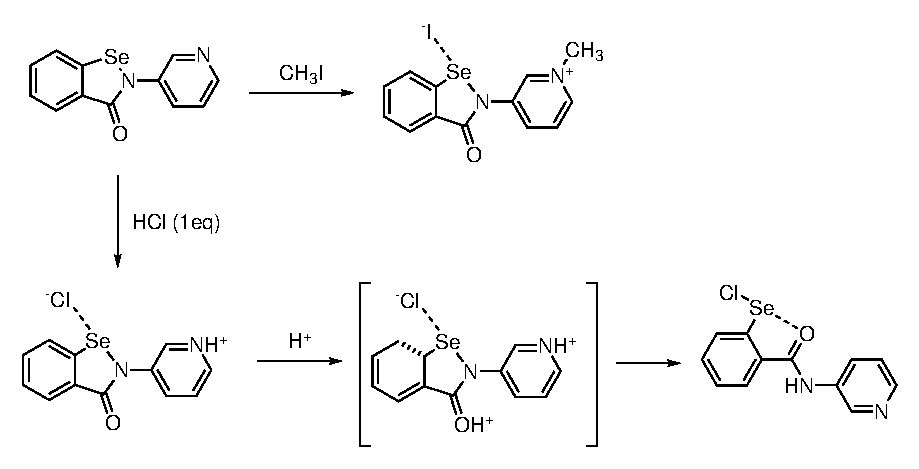
\includegraphics[scale=0.8]{Figures/scheme.eps}
    \caption{Reactions of 3-pyridyl ebselen \refcmpd{ebs.3py}.}
    \label{sch:selenylchloride-mechanism}
\end{figure}

\begin{figure}
    \centering
    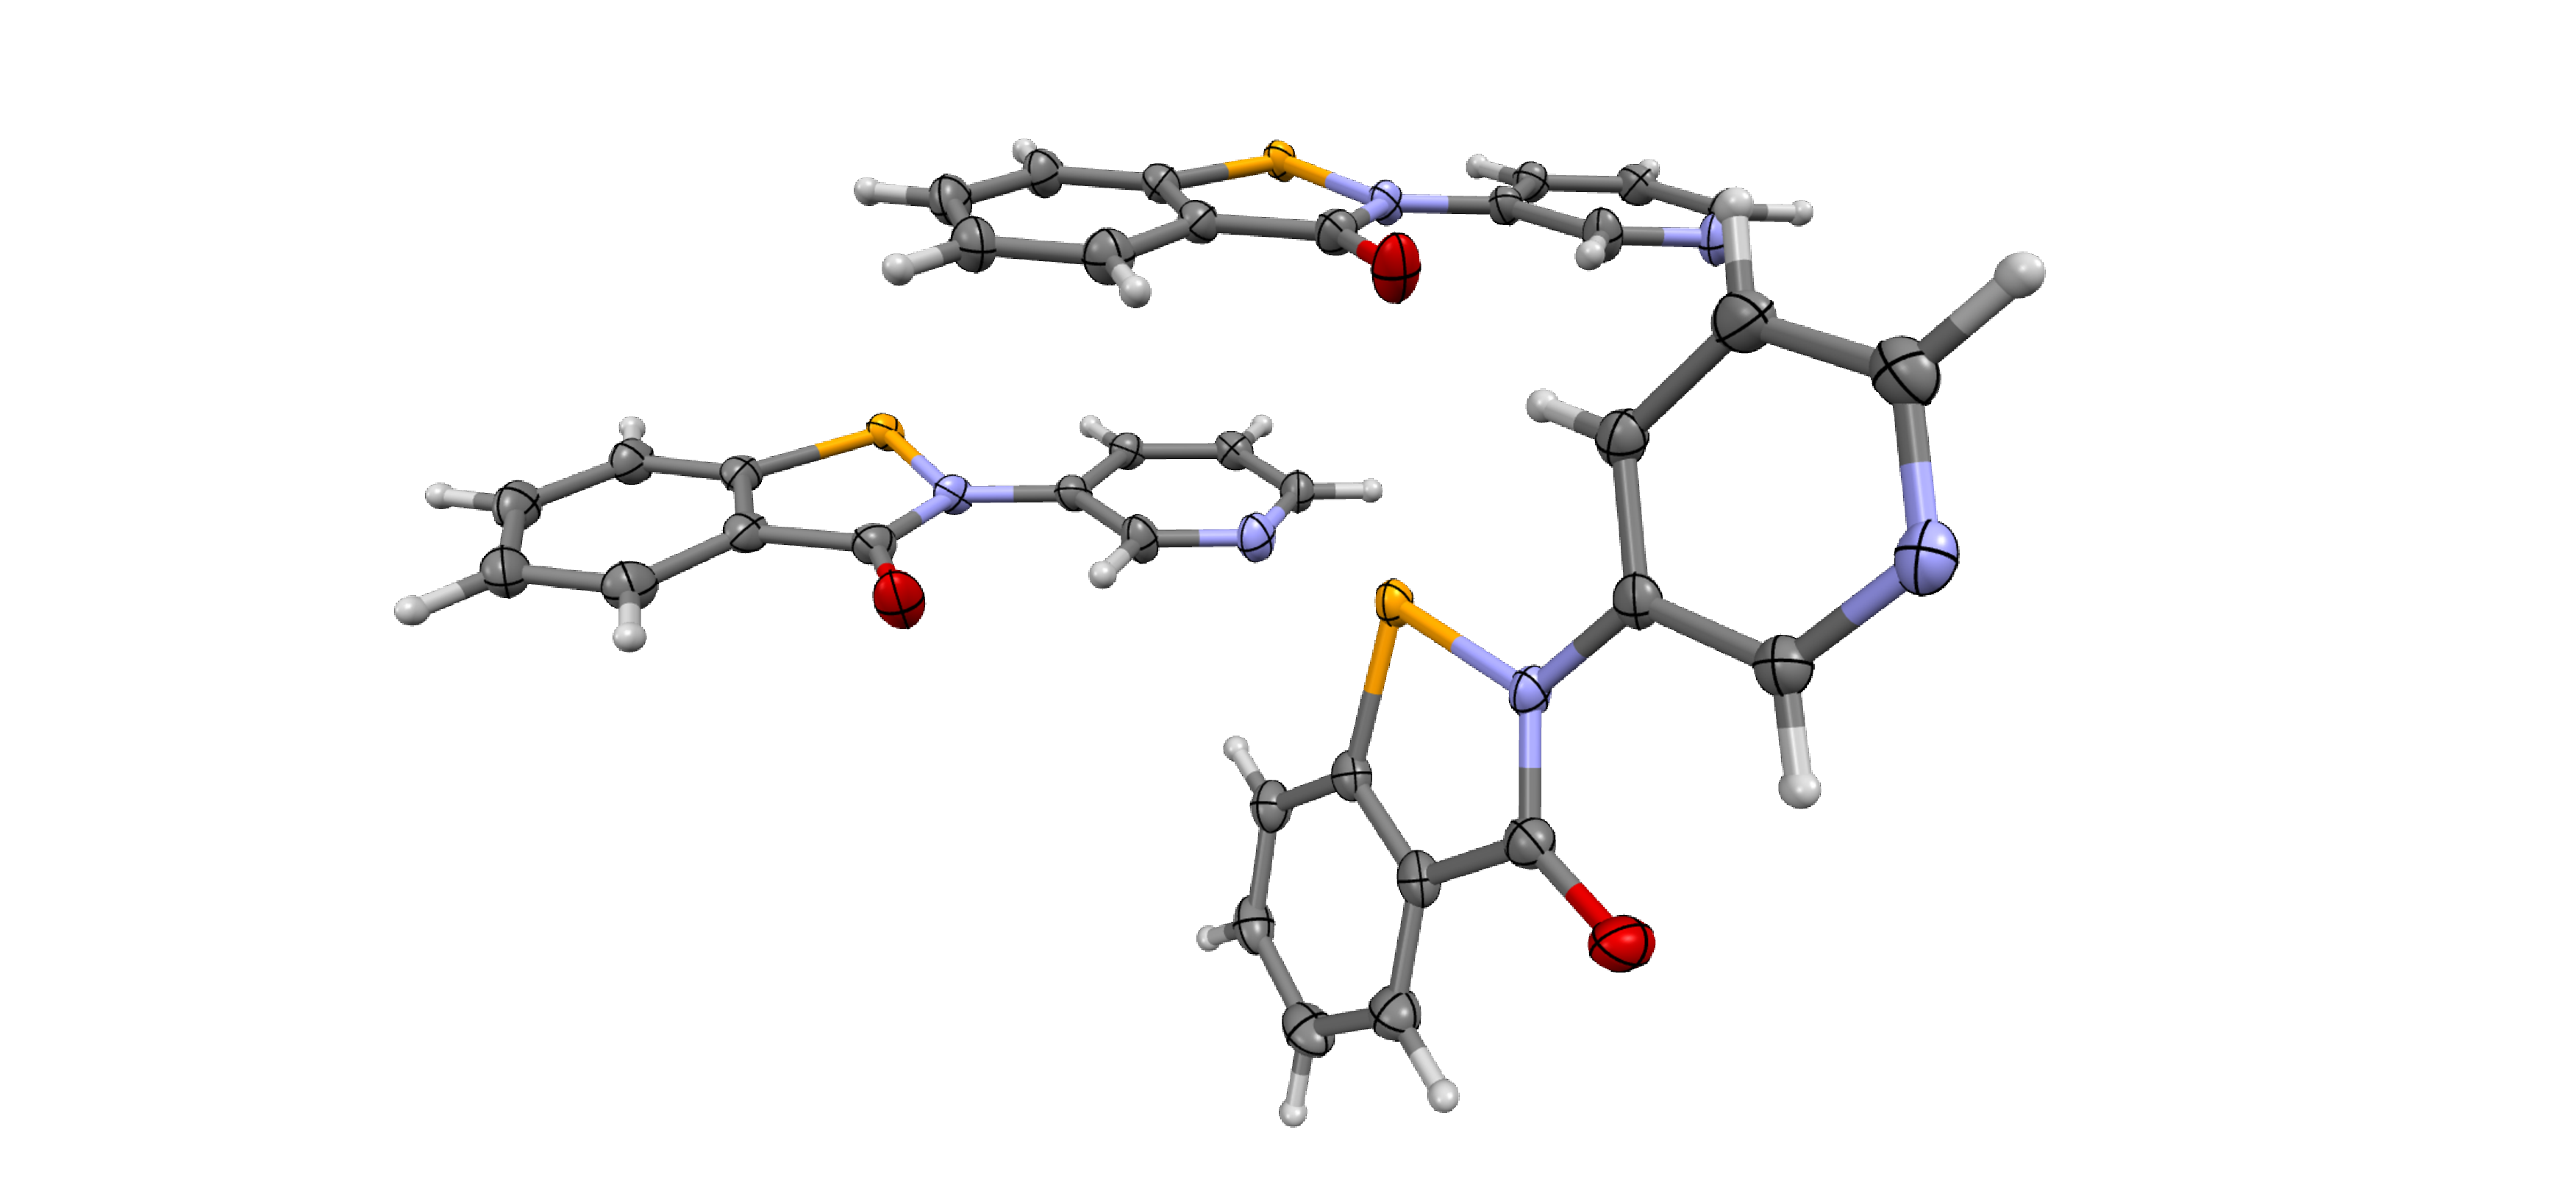
\includegraphics[width=\linewidth]{Figures/3py-ebs-chbonds.pdf}
    \caption{Ch-bonds formed by 3-pyridyl ebselen \refcmpd{ebs.3py} in the crystal packing. The stronger of the two is defined by the \ce{N-Se\cdots N_{pyr}} angle, and the weaker is defined by the \ce{C-Se\cdots O} angle.}
    \label{fig:3py-ebs-chbonds}
\end{figure}

\begin{figure}
    \centering
    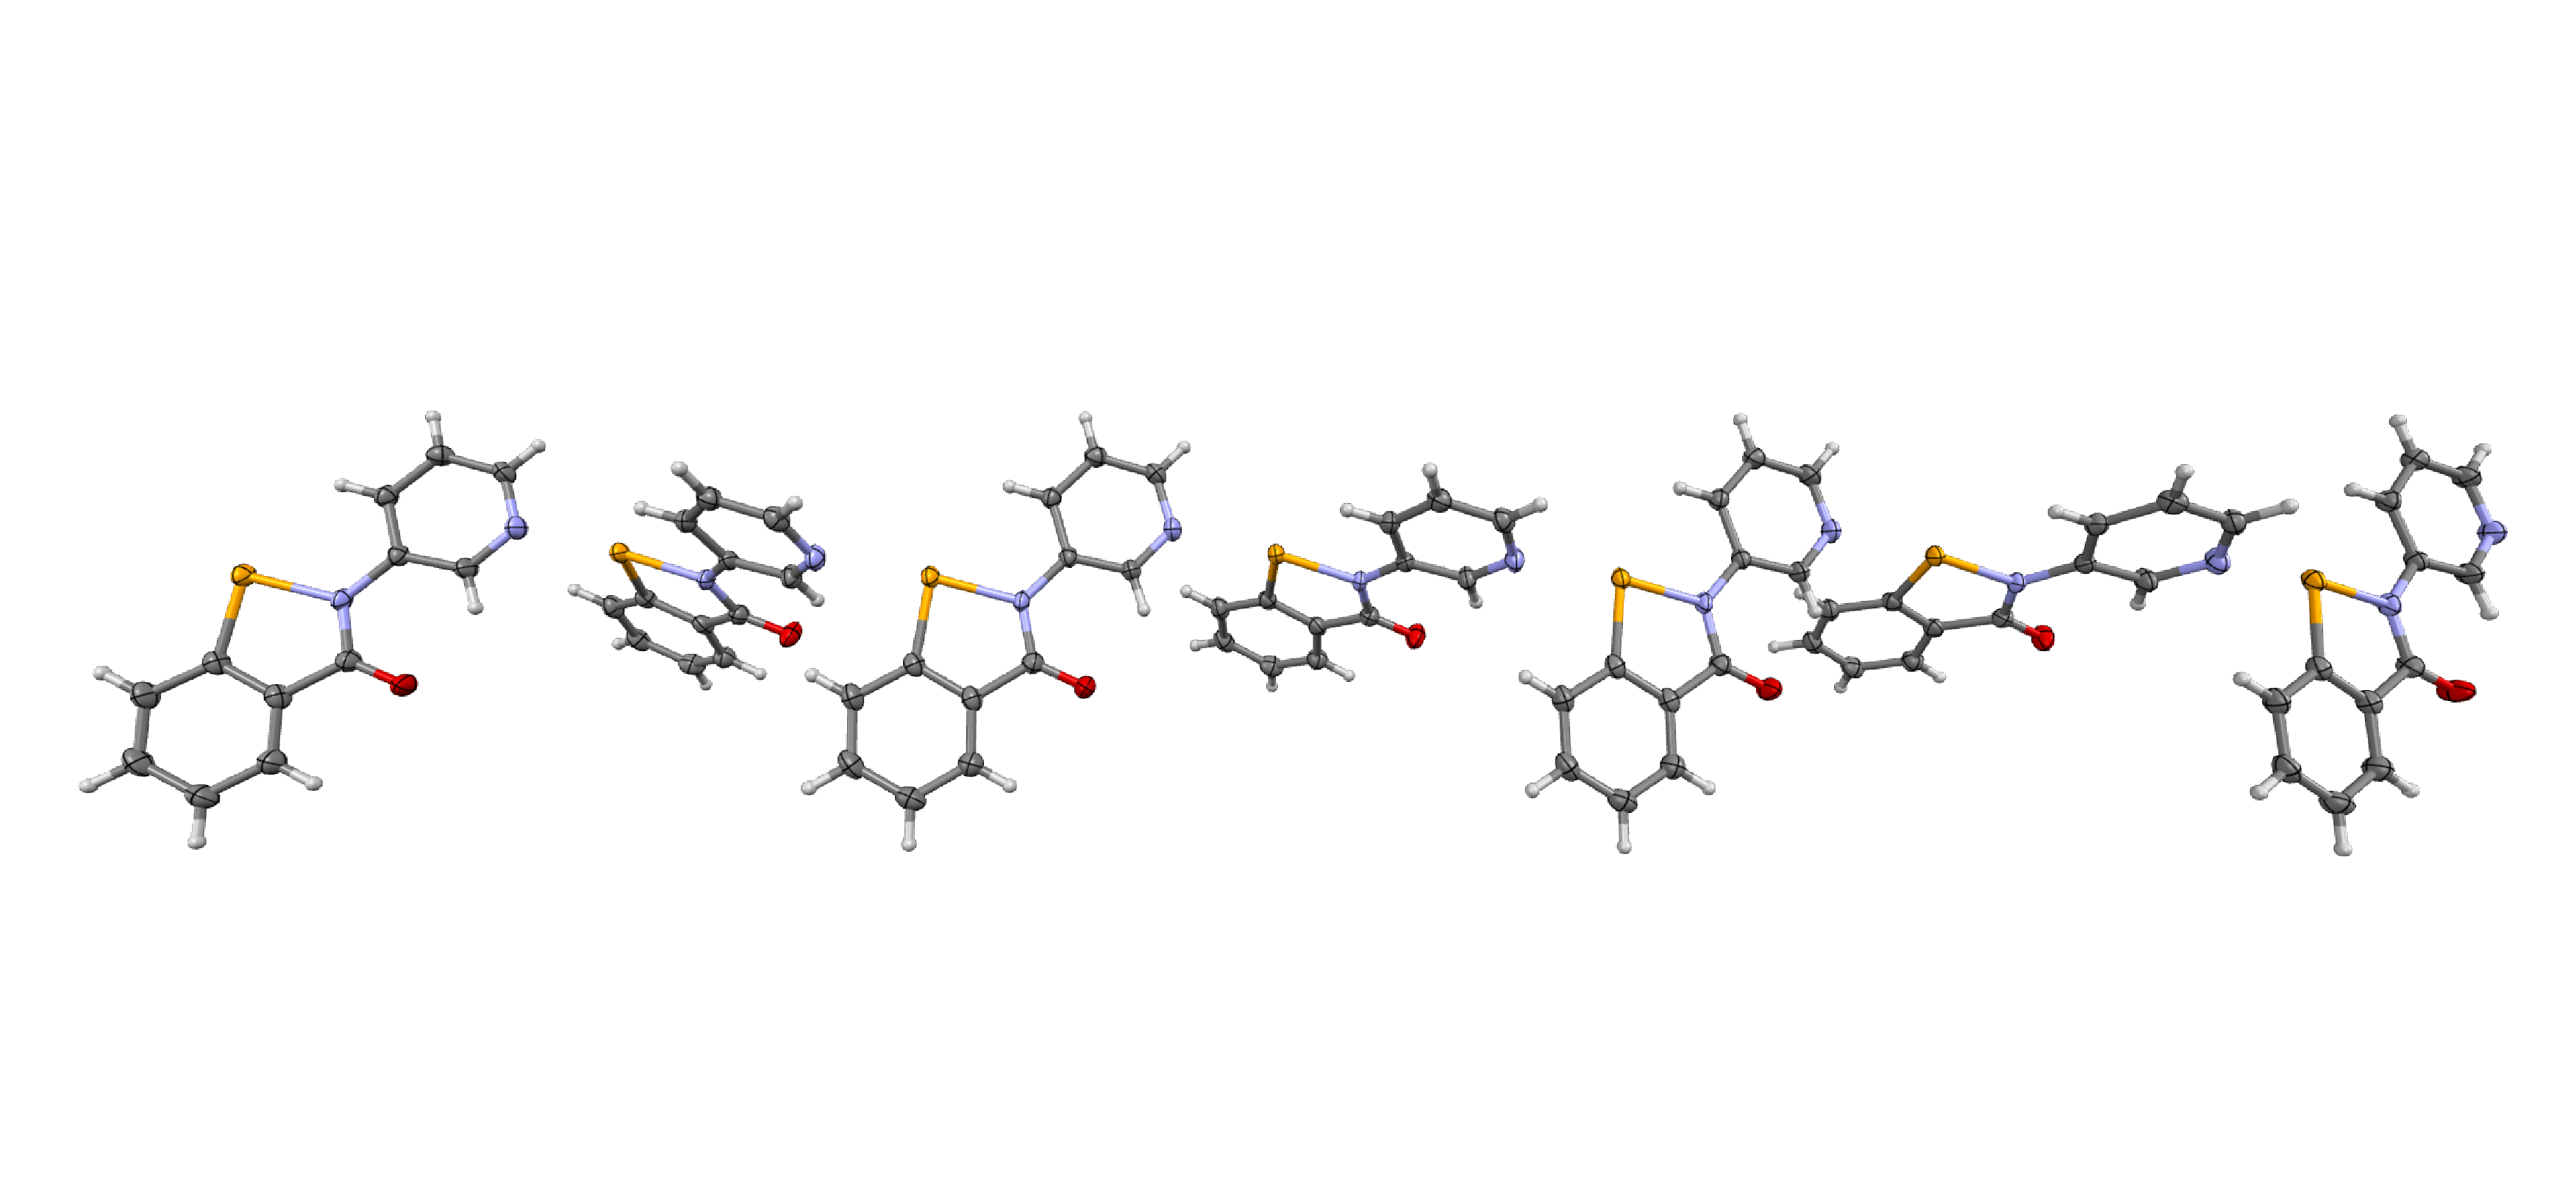
\includegraphics[width=\linewidth]{Figures/3py-ebs-chain.pdf}
    \caption{One-dimensional network formed by the strong \ce{N-Se\dots N} Ch-bonds. This is extended into 3 dimensions by the weaker \ce{C-Se\dots O} Ch-bonds, and $\pi$-stacking.}
    \label{fig:3py-ebs-chain}
\end{figure}

\begin{figure}
    \centering
    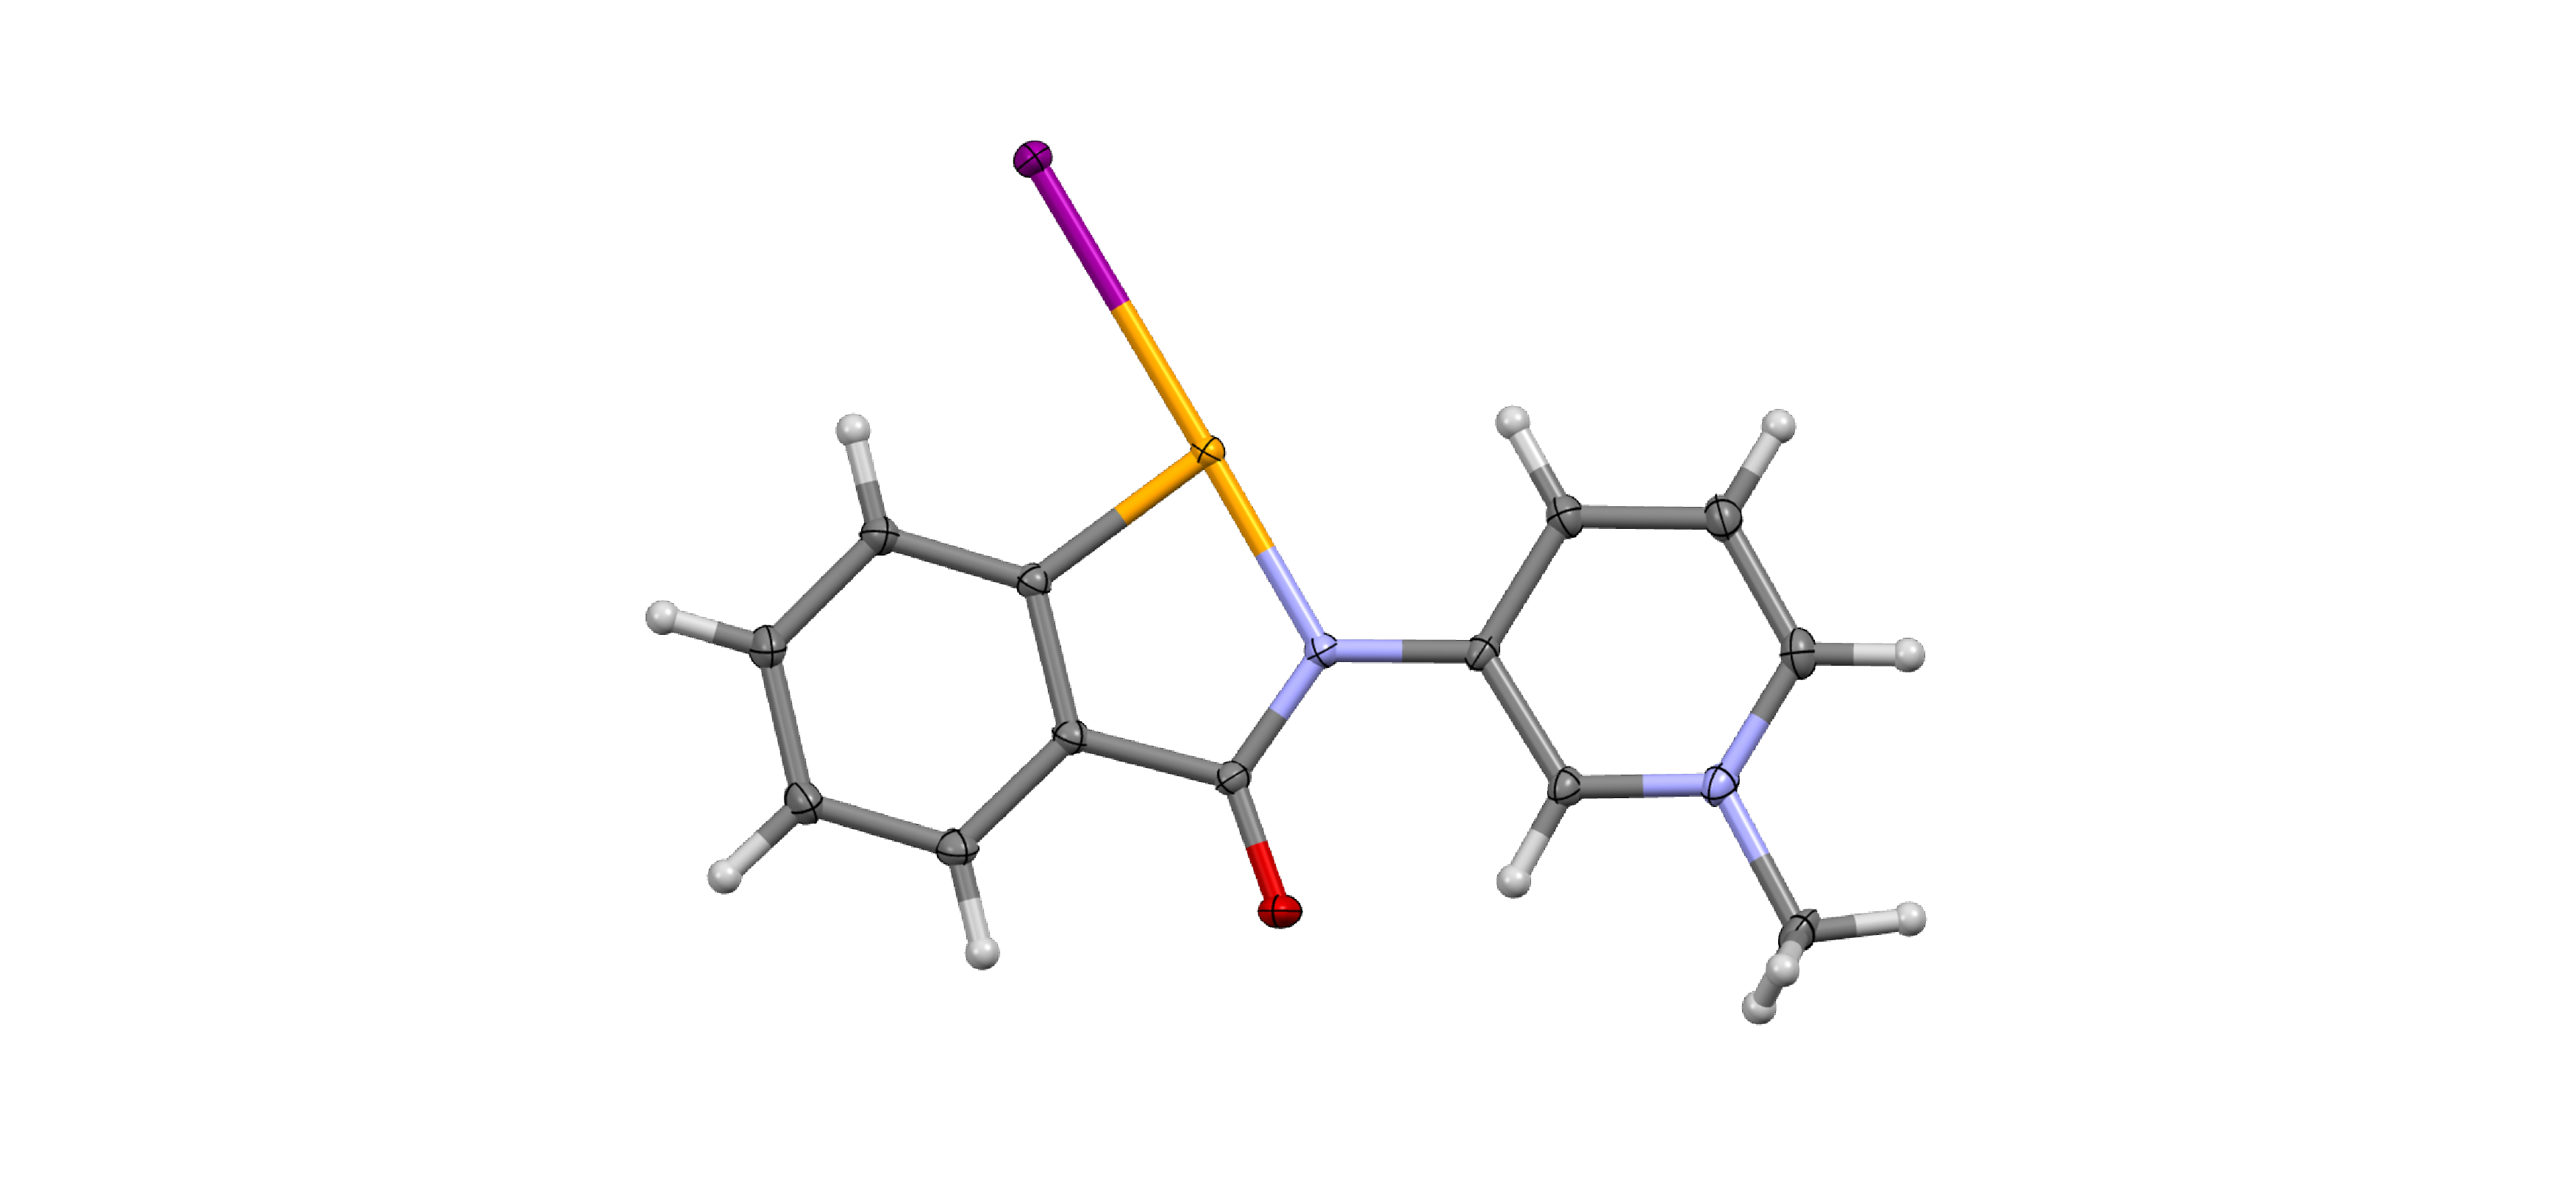
\includegraphics[width=0.6\linewidth]{Figures/3py-ebs-mei.pdf}
    \caption{Structure of the methylated derivative \refcmpd{ebs.me3py}.}
    \label{fig:3py-ebs-mei}
\end{figure}

\begin{figure}
    \centering
    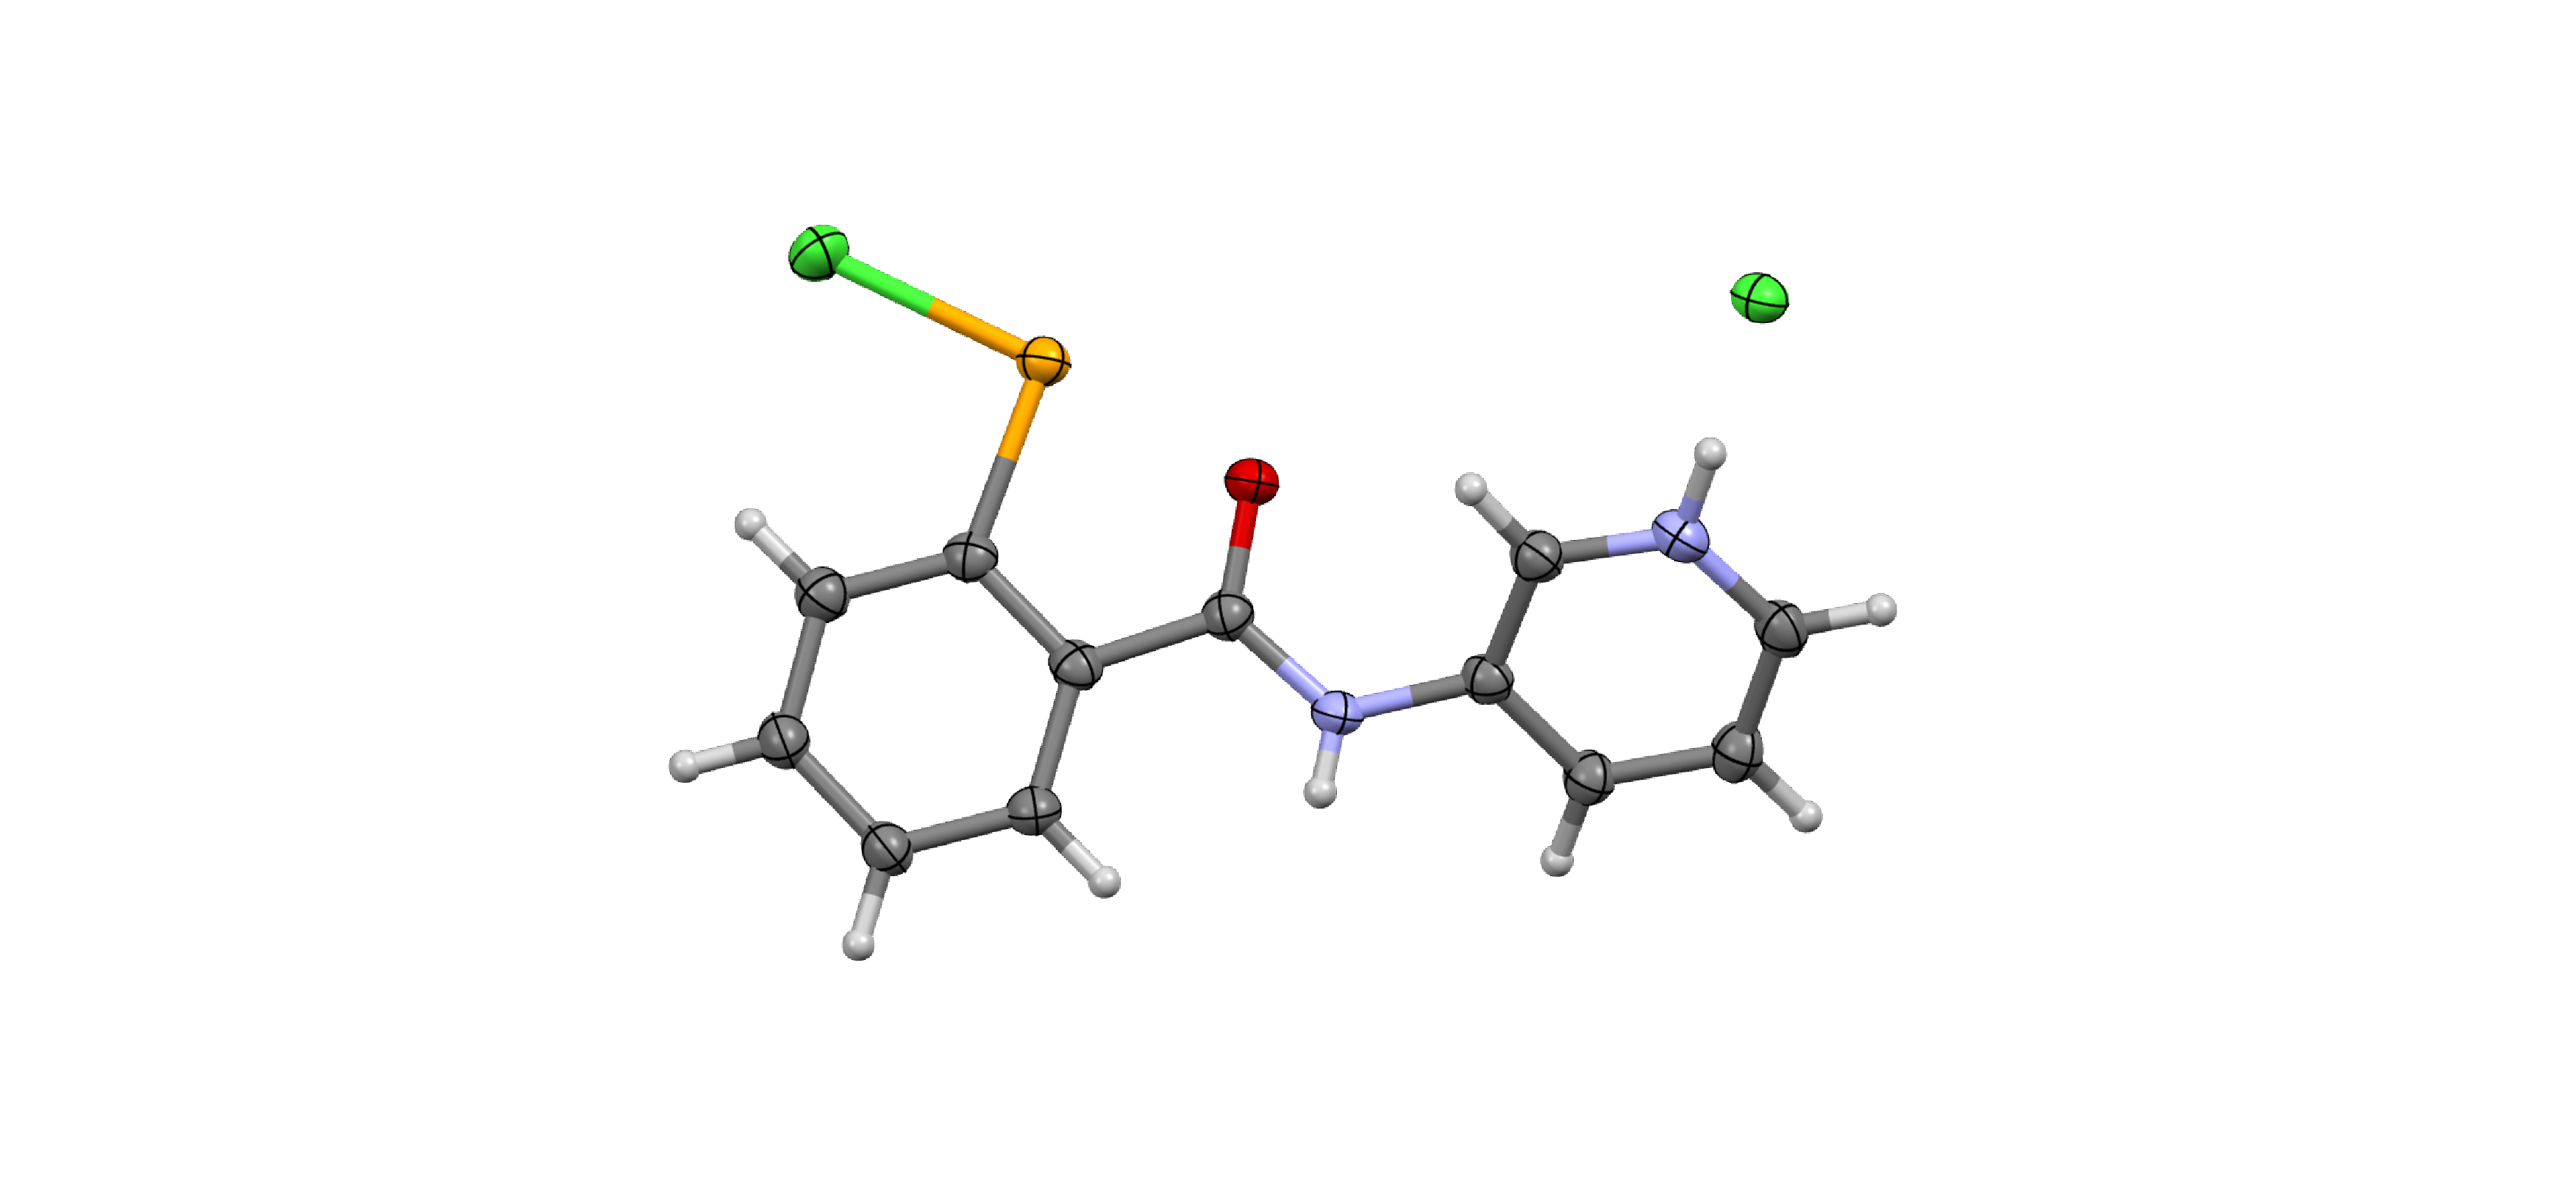
\includegraphics[width=0.6\linewidth]{Figures/3py-ebs-hcl.pdf}
    \caption{Structure of the ring opened hydrochloride derivative \refcmpd{selenylchloride-3py}.}
    \label{fig:3py-ebs-hcl}
\end{figure}

%\printbibliography[heading=subbibliography]
\end{refsection}

\begin{refsection}

\chapter{Development of a Ch-bonding DNA binder}
\section{Introduction}

\subsection{Mechanism of radioprotection}
The mechanism by which bis-benzimidazoles impart radioprotection is believed to be a proton coupled electron transfer from the bound ligand to the damaged DNA.\cite{???}
This was elucidated from a structure-activity relationship study, where it was observed that the acidity of the $1^\prime$ proton was strongly correlated with radioprotective ability.

Ebselen itself, of course, displays antioxidant properties too.
These are believed to be the basis for its neuroprotective, anti-helmenthic, and anti-inflammatory behaviour.\cite{???}
The mechanism, however, appears to be completely different. 
Ebselen behaves as a glutathione peroxidase mimic, that is to say, a catalyst that increases the rate at which glutathione reduces reactive oxygen species.

\begin{scheme}
\replacecmpd{rhs-nitro-amide}
\replacecmpd{rhs-nitro}
\replacecmpd{rhs-amine}
\replacecmpd{ebs-rhs}
\caption{Synthesis of benzisoselenazolone-benzimidazole Hoechst analogue \refcmpd{ebs-rhs}.}
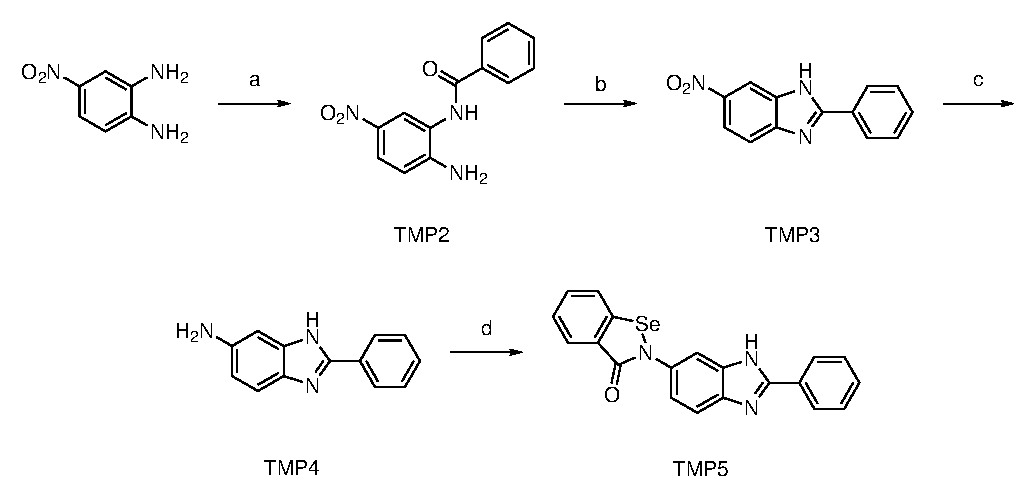
\includegraphics[scale=0.8]{Figures/ebs-rhs-synthesis.eps}
\label{sch:ebs-rhs-synthesis}
\end{scheme}

\begin{scheme}
\replacecmpd{2cl-4no2-amide}
\replacecmpd{ebs-3no2}
\replacecmpd{ebs-3nh2}
\replacecmpd{ebs-ebs}
\caption{Synthesis of bis-benzisoselenazolone Hoechst analogue \refcmpd{ebs-ebs}.}
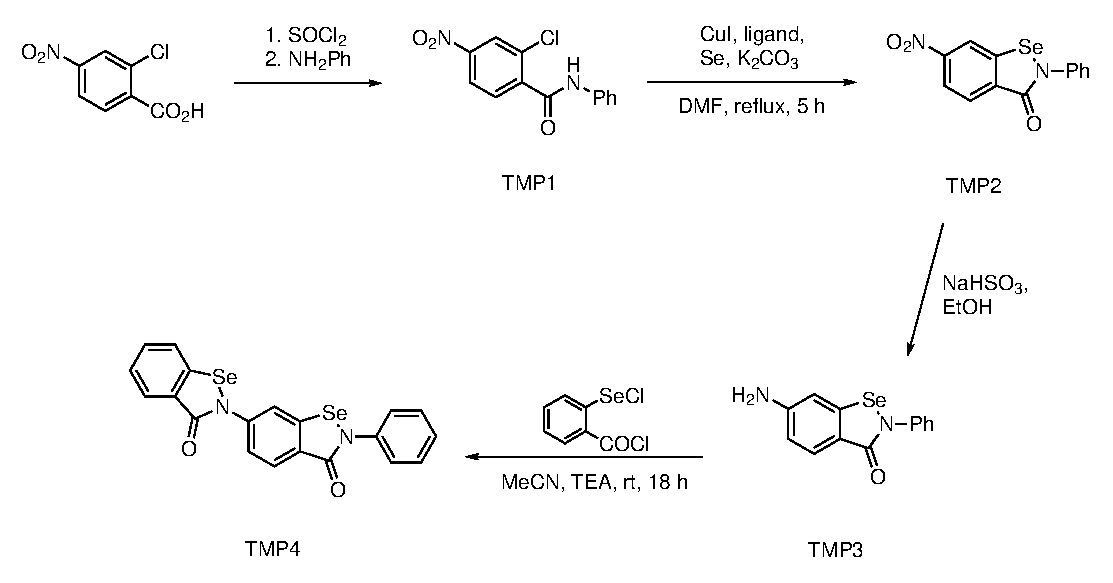
\includegraphics[scale=0.8]{Figures/ebs-ebs-synthesis.eps}
\label{sch:ebs-ebs-synthesis}
\end{scheme}


\section{\emph{In silico} modelling}

\section{Synthesis of analogues}

\section{DNA binding studies}


\section{Conclusions}


\section{Experimental procedures}


\subsection{Synthetic methods}

Selenium was purified by refluxing in 32\% hydrochloric acid for 2~h, then washing with methanol and ether.

\subsubsection{Preparation of N-(2-amino-5-nitrophenyl)benzamide \refcmpd{rhs-nitro-amide}}
4-Nitro-1,2-benzenediamine (3.0797~g, 20.110~mmol) and TEA (3~mL, distilled from \ce{CaH2}) were dissolved in anhydrous THF (150~mL).
Benzoyl chloride (1.5~mL, 1.8~g, 13~mmol) was then added at $-10$\degree C and the mixture slowly warmed to room temperature while stirring for 18~h.
The mixture was then tipped into water (400~mL), and extracted with ethyl acetate ($3\times100$~mL).
The combined organic layers were washed with water ($2\times200$~mL), brine (200~mL), then dried (\ce{MgSO4}) and evaporated to give a reddish solid.
This was recrystallised from ethyl acetate to give the amide \cmpd{rhs-nitro-amide} as yellow crystals (2.5027~g, 75\%).

\ce{^1H} NMR (400~MHz, DMSO-\emph{d6}) $\delta$ 9.66 (s, 1H), 8.04 (s, 1H), 7.92 (d, J = 7.4 Hz, 2H), 7.83 (d, J = 9.2 Hz, 1H), 7.50 (d, J = 6.8 Hz, 1H), 7.44 (t, J = 7.3 Hz, 2H), 6.71 (d, J = 9.0 Hz, 1H), 6.52 (s, 2H). 

\subsubsection{Preparation of 6-nitro-2-phenyl-1\emph{H}-benzo[\emph{d}]imidazole \refcmpd{rhs-nitro}}
%TF-7-94-CP
Amide \cmpd{rhs-nitro-amide} (1.2283~g, 4.7749~mmol) was refluxed in a solution of \ce{BF3\cdot OEt2} (0.75~mL) and dioxane (75~mL) for 1.5~h. 
The mixture was then cooled to room temperature, stirred for 18~h, then heated to reflux again for 2~h.
The yellow solution was diluted with water (300~mL) and extracted with ethyl acetate ($3\times75$~mL),
The combined organic layers were washed with water and brine (100~mL each), then dried (\ce{Na2SO4}), and evaporated to give a brown oil.
Trituration with petroleum spirit/dichloromethane afforded \cmpd{rhs-nitro} as a light brown friable solid (1.0606~g, 93\%).

\ce{^1H} NMR (400~MHz, DMSO-\emph{d6}) $\delta$ 8.47 (s, 1H), 8.21 (q, J = 3.2 Hz, 2H), 8.13 (q, J = 3.7 Hz, 1H), 7.76 (d, J = 8.9 Hz, 1H), 7.54--7.62 (m, 3H). 

\begin{figure}[h]
    \centering
    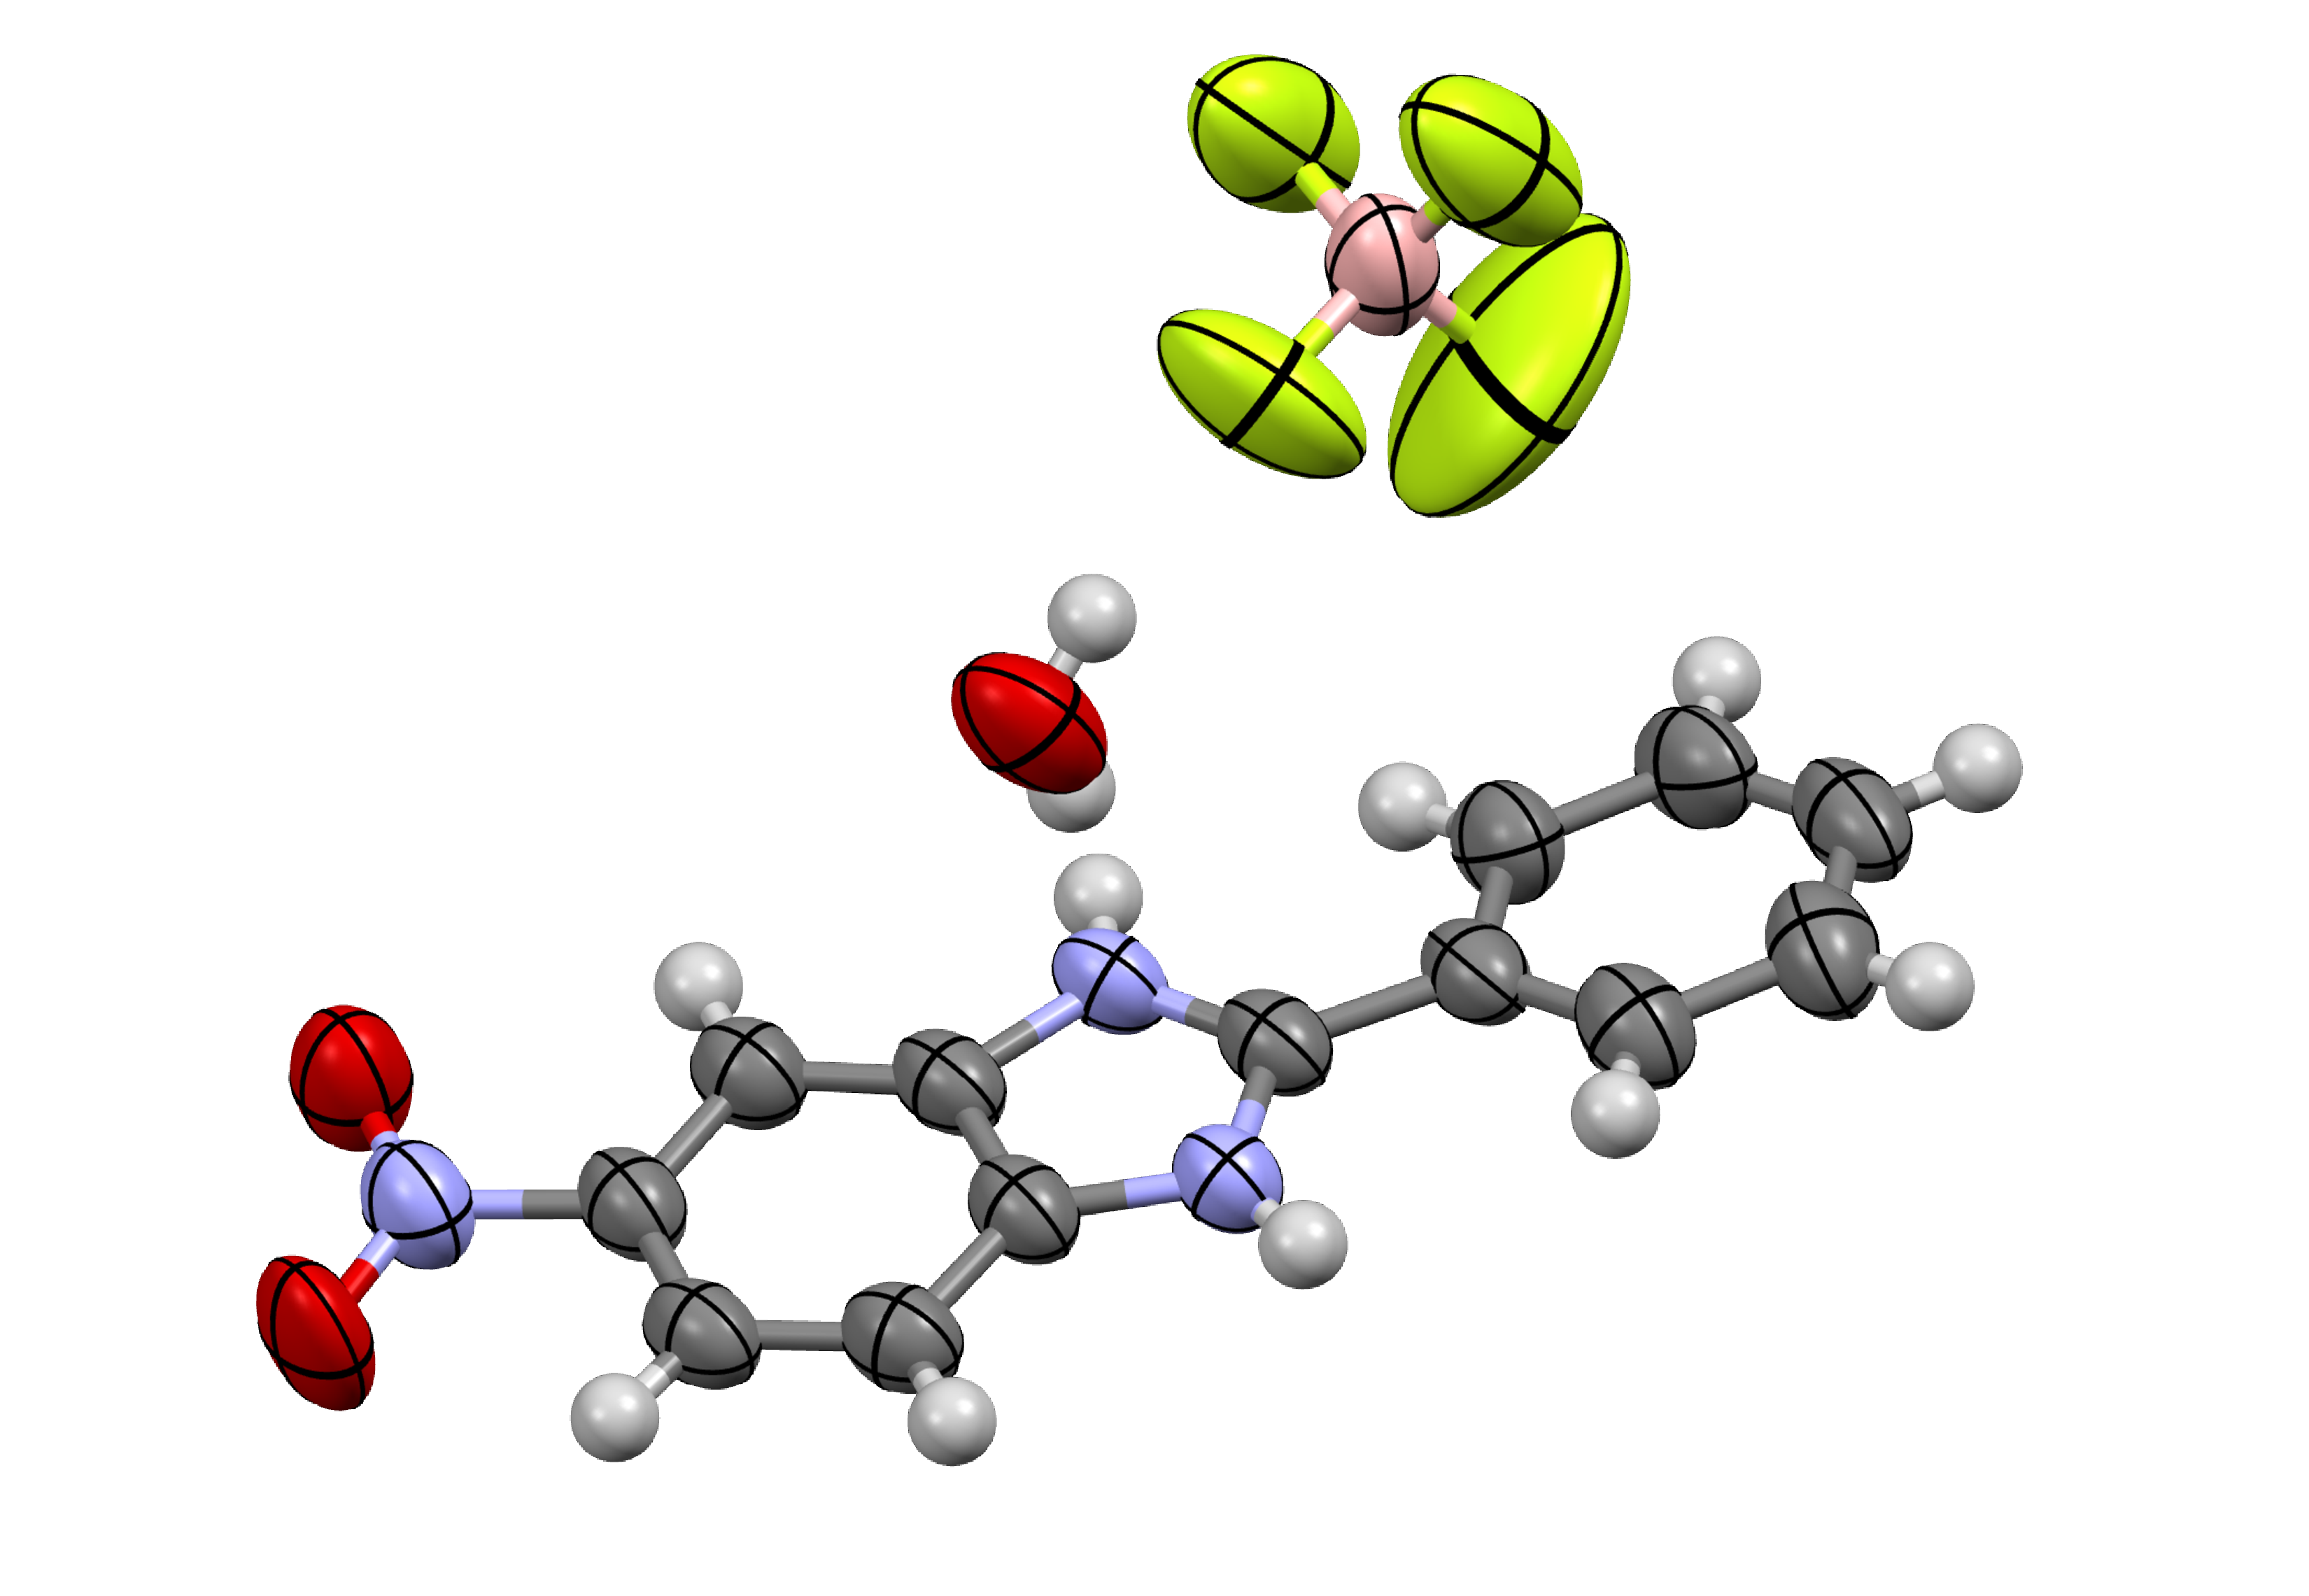
\includegraphics[width=0.8\linewidth]{Figures/rhs-nitro-xray.pdf}
    \caption{X-ray crystal structure of \refcmpd{rhs-nitro} as the tetrafluoroborate salt.}
    \label{fig:rhs-nitro-xray}
\end{figure}

\subsubsection{Preparation of 2-phenyl-1\emph{H}-benzo[\emph{d}]imidazol-6-amine \refcmpd{rhs-amine}}
%TF-7-117-CP
A solution of the nitrobenzene \cmpd{rhs-nitro} (893.6~mg, 3.735~mmol) and tin (II) chloride dihydrate (4.410~g, 19.54~mmol) in concentrated hydrochloric acid (20~mL) was refluxed for 2~h. 
The solution was then cooled, and basified to pH 10 using 5~M aqueous sodium hydroxide.
This was then extracted with ethyl acetate ($2\times30$~mL), washing with water and brine (30~mL each).
The combined organic layers were dried (\ce{Na2SO4}) then evaporated to give \cmpd{rhs-amine} as a brownish solid (677.2~mg, 87\%).

\begin{figure}[h]
    \centering
    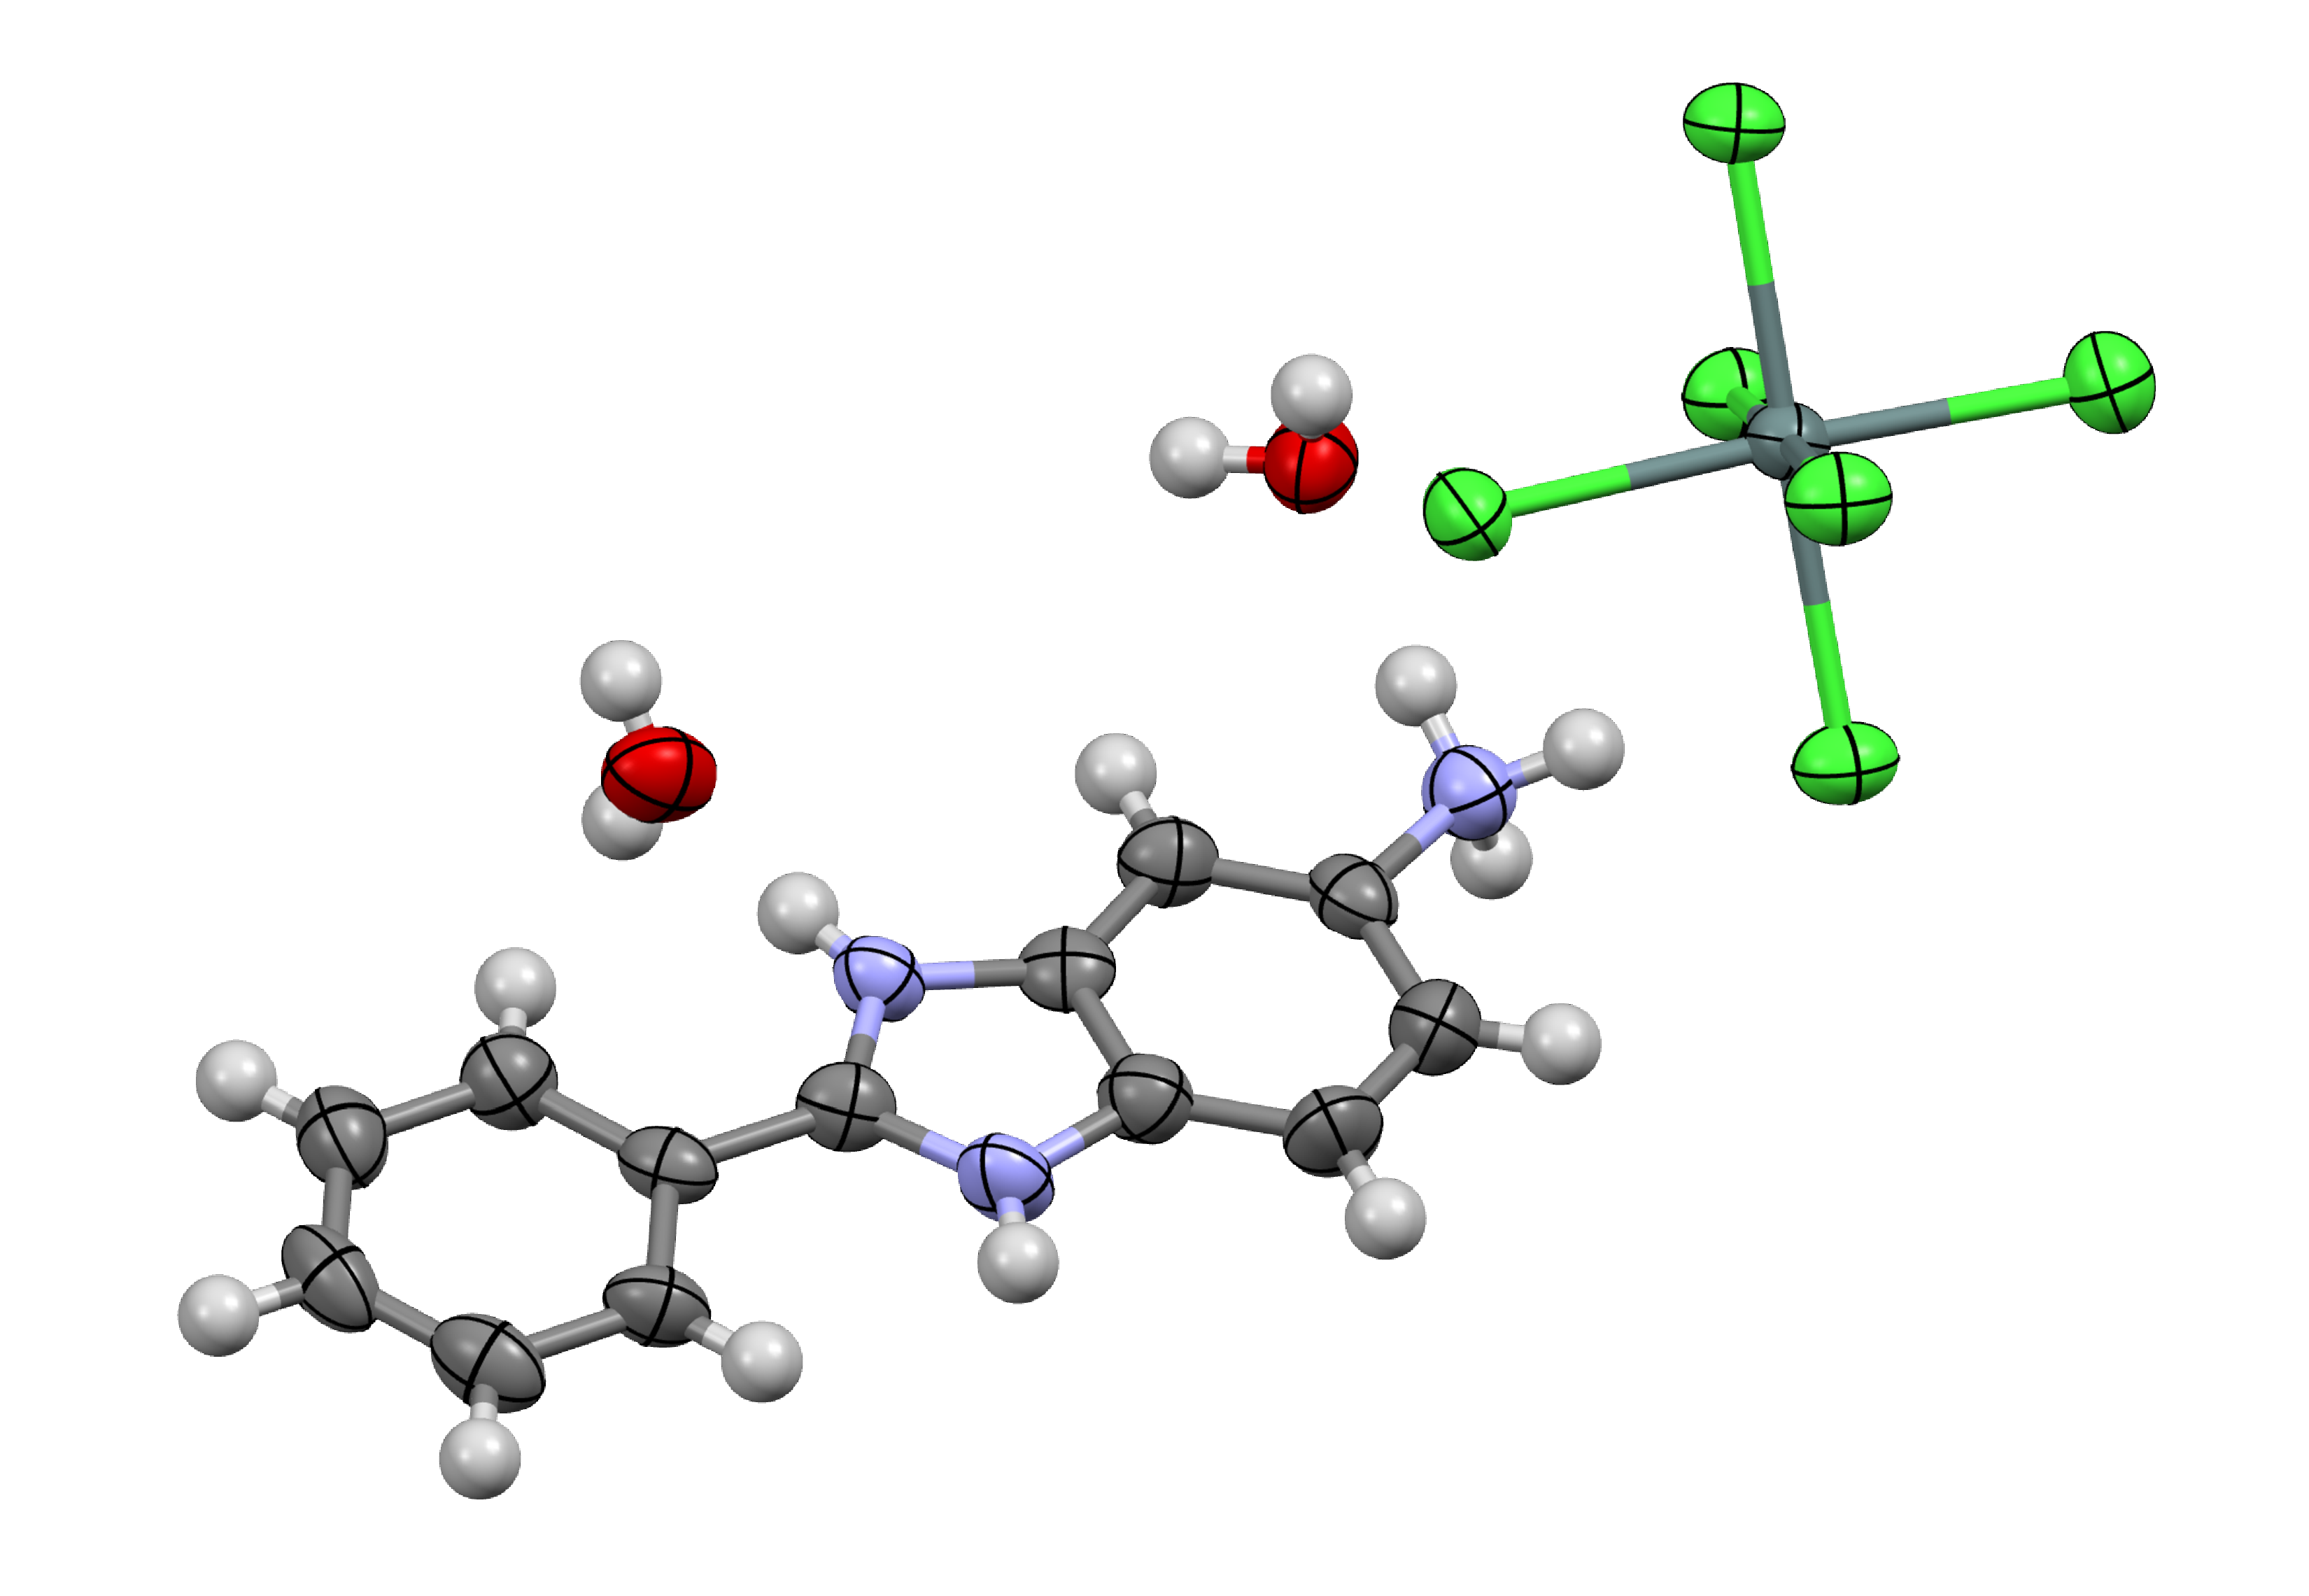
\includegraphics[width=0.8\linewidth]{Figures/rhs-amine-xray.pdf}
    \caption{X-ray crystal structure of \refcmpd{rhs-amine} as the hexachlorostannate salt.}
    \label{fig:rhs-amine-xray}
\end{figure}

\subsubsection[Preparation of \refcmpd{ebs-rhs}]{Preparation of 2-(2-phenyl-1\emph{H}-benzo[\emph{d}]imidazol-6-yl)benzo[\emph{d}][1,2]selenazol-3(2\emph{H})-one \refcmpd{ebs-rhs}}
%TF-7-188-C1F1
Diselenide \cmpd{diselenide} (440.1~mg, 1.100~mmol) was refluxed in thionyl chloride with 2 drops DMF for 2~h. 
The excess reagent was removed by vacuum distillation, and the residue was dissolved in anhydrous acetonitrile (10~mL).
This was added dropwise to a solution of the aniline \cmpd{rhs-amine} (440.4~mg, 2.105~mmol) and TEA (2~mL) in a further 10~mL anhydrous acetonitrile.
The mixture was stirred at room temperature for 18~h, then briefly brought to reflux.
It was then cooled, diluted with water (30~mL) and extracted into ethyl acetate ($3\times50$~mL).
The combined organic layers were washed with water and brine (50~mL each), then dried (\ce{MgSO4}), then evaporated onto celite.
This was chromatographed on a SNAP 25~g silica cartridge using an ethyl acetate/methanol gradient, affording 2 major fractions:
\begin{enumerate}
    \item orange solid, 67.7~mg, 8\%, \cmpd{ebs-rhs}
    \item yellow solid, 166.0~mg, 38\%, starting material \cmpd{rhs-amine}
\end{enumerate}

\begin{figure}[h]
    \centering
    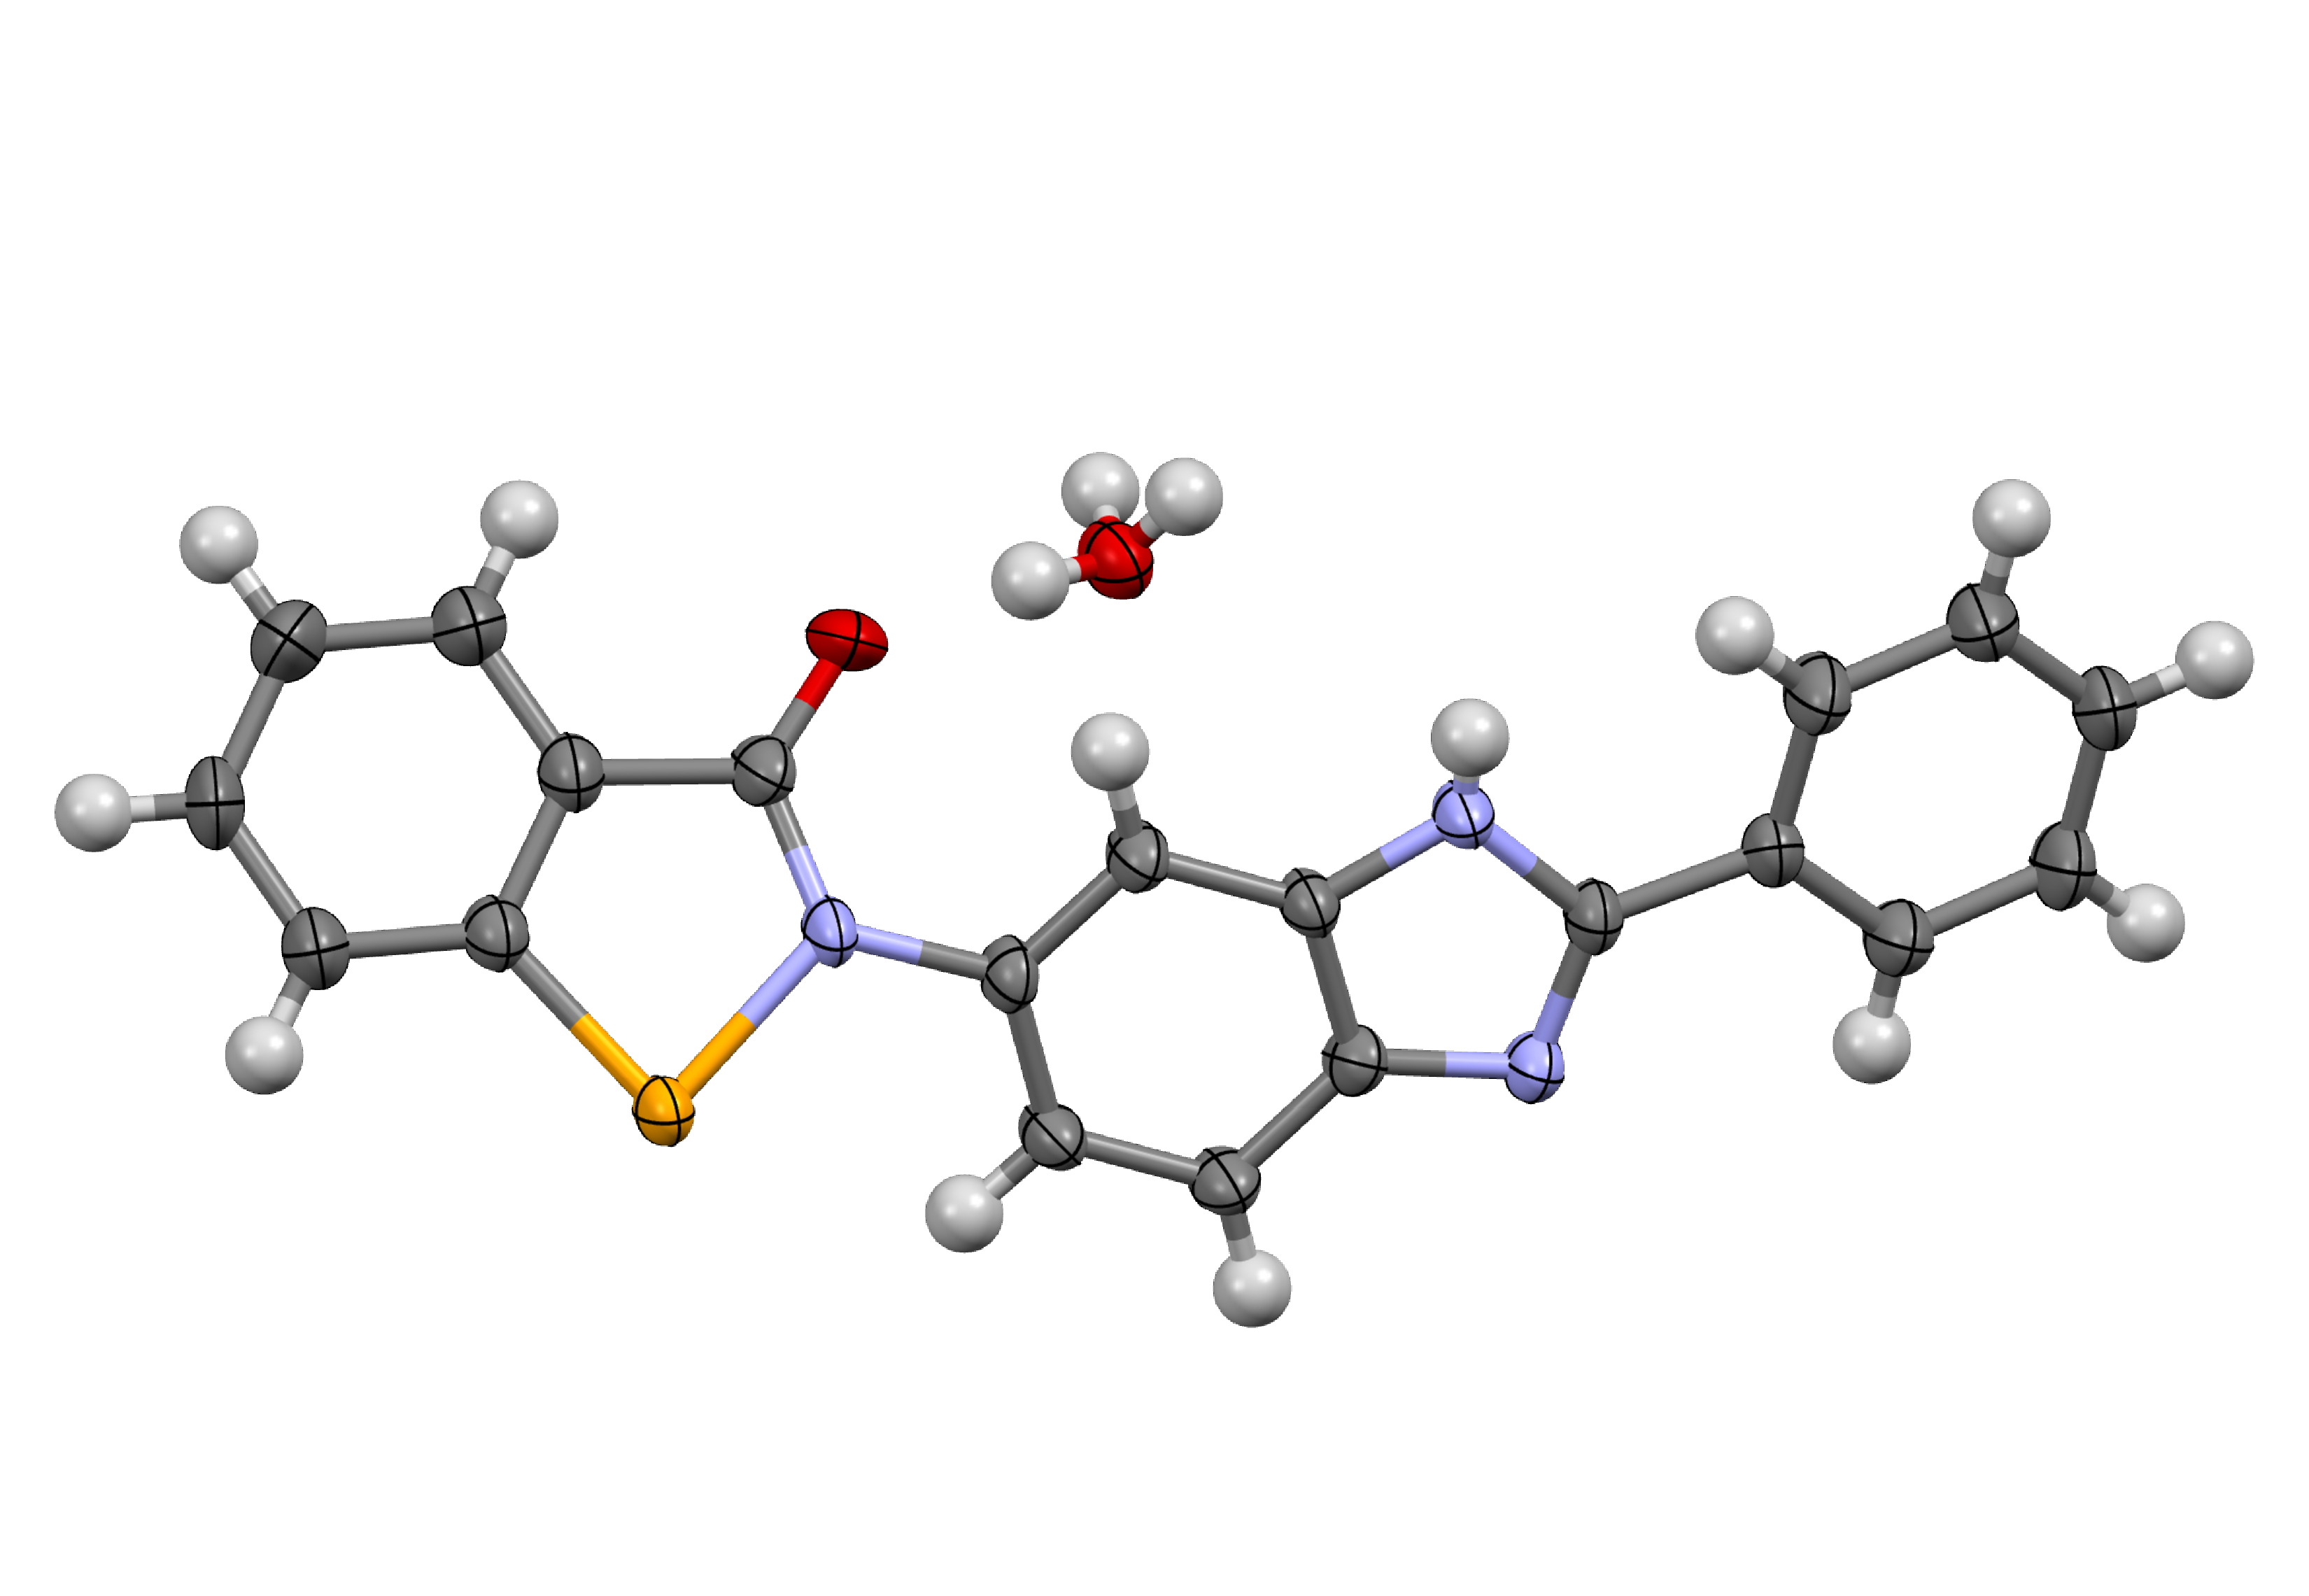
\includegraphics[width=0.8\linewidth]{Figures/ebs-rhs-xray.pdf}
    \caption{X-ray crystal structure of \refcmpd{ebs-rhs}. The water is disordered over 3 sites, with each proton having an occupancy of 2/3.}
    \label{fig:ebs-rhs-xray}
\end{figure}

\subsubsection{Preparation of 2-chloro-4-nitro-\emph{N}-phenylbenzamide \refcmpd{2cl-4no2-amide}}
%TF-7-128-recryst
2-Chloro-4-nitrobenzoic acid (10.3144~g, 51.173~mmol) was refluxed in thionyl chloride (20~mL) with 3 drops DMF for 2~h. 
The excess reagent was then removed by vacuum distillation and the residue was dissolved in anhydrous DCM (100~mL).
This was added slowly to a solution of aniline (4.756~g, 51.07~mmol) and TEA (10~mL, distilled from \ce{CaH2}) in a further 100~mL of anhydrous DCM.
The mixture was stirred for 18~h at room temperature, then the solvent was removed \emph{in vacuo}.
The residue was washed with water ($3\times$50~mL), then recrystallised from ethanol to afford \cmpd{2cl-4no2-amide} as colourless plates (10.5134~g, 75\%).

\footnotesize\paragraph{}

\ce{^{1}H} NMR (500~MHz, \ce{CDCl3}) $\delta$ ppm
7.23 (t, J=7.48 Hz, 1 H), 
7.42 (t, J=7.78 Hz, 2 H), 
7.64 (d, J=7.93 Hz, 2 H), 
7.81 (br. s., 1 H), 
7.93 (d, J=8.39 Hz, 1 H), 
8.24 (d, J=8.39 Hz, 1 H), 
8.35 (d, J=1.07 Hz, 1 H).

\normalsize

\subsubsection[Preparation of \refcmpd{ebs-3no2}]{Preparation of 6-nitro-2-phenylbenzo[\emph{d}][1,2]selenazol-3(2\emph{H})-one \refcmpd{ebs-3no2}}
Copper (I) iodide (127.2~mg, 0.6679~mmol) and 1,10-phenanthroline (121.5~mg, 0.6743~mmol) were dissolved in anhydrous DMF (4~mL).
To this was added selenium (1035.1~mg, 13.109~mmol) and potasssium carbonate (755.9~mg, 5.469~mmol), and the mixture heated to 120\degree C under a nitrogen atomsphere for 5~min.
The mixture was then cooled, the amide \cmpd{2cl-4no2-amide} (968.4~mg, 3.500~mmol) added, and the mixture was again heated at 120\degree C under nitrogen for 18~h.
Upon cooling, the mixture was tipped into brine (200~mL) and stirred in the air for 3~h, then extracted into ethyl acetate ($4\times50$~mL).
The combined organic phases were washed with water then brine (100~mL each), then dried (\ce{MgSO4}) and evaporated to give a dark orange solid.
This was redissolved in ethanol (70~mL) and cooled to $-20$\degree C for 72~h, affording \cmpd{ebs-3no2} as an orange precipitate, which was filtered and dried (119.1~mg, 11\%, m.p. 256.2--258.2\degree C (dec.)).
The mother liquor was loaded onto silica and chromatographed using a SNAP 50~g silica cartridge, affording 3 major fractions which were not further characterised.

{\footnotesize
\ce{^{1}H} NMR (400~MHz, \ce{\emph{d}6}-DMSO) $\delta$ ppm
.

\ce{^{13}C} NMR (100~MHz, \ce{\emph{d}6}-DMSO) $\delta$ ppm
.

\ce{^{77}Se} NMR (0~MHz, \ce{\emph{d}6}-DMSO) $\delta$ ppm
.

MS (ESI +ve) m/z 320.97720 (\ce{MH+}) \ce{C13H9N2O3Se+} requires 320.97729 ($\Delta$=-0.09~mmu).
}

\begin{figure}[h]
    \centering
    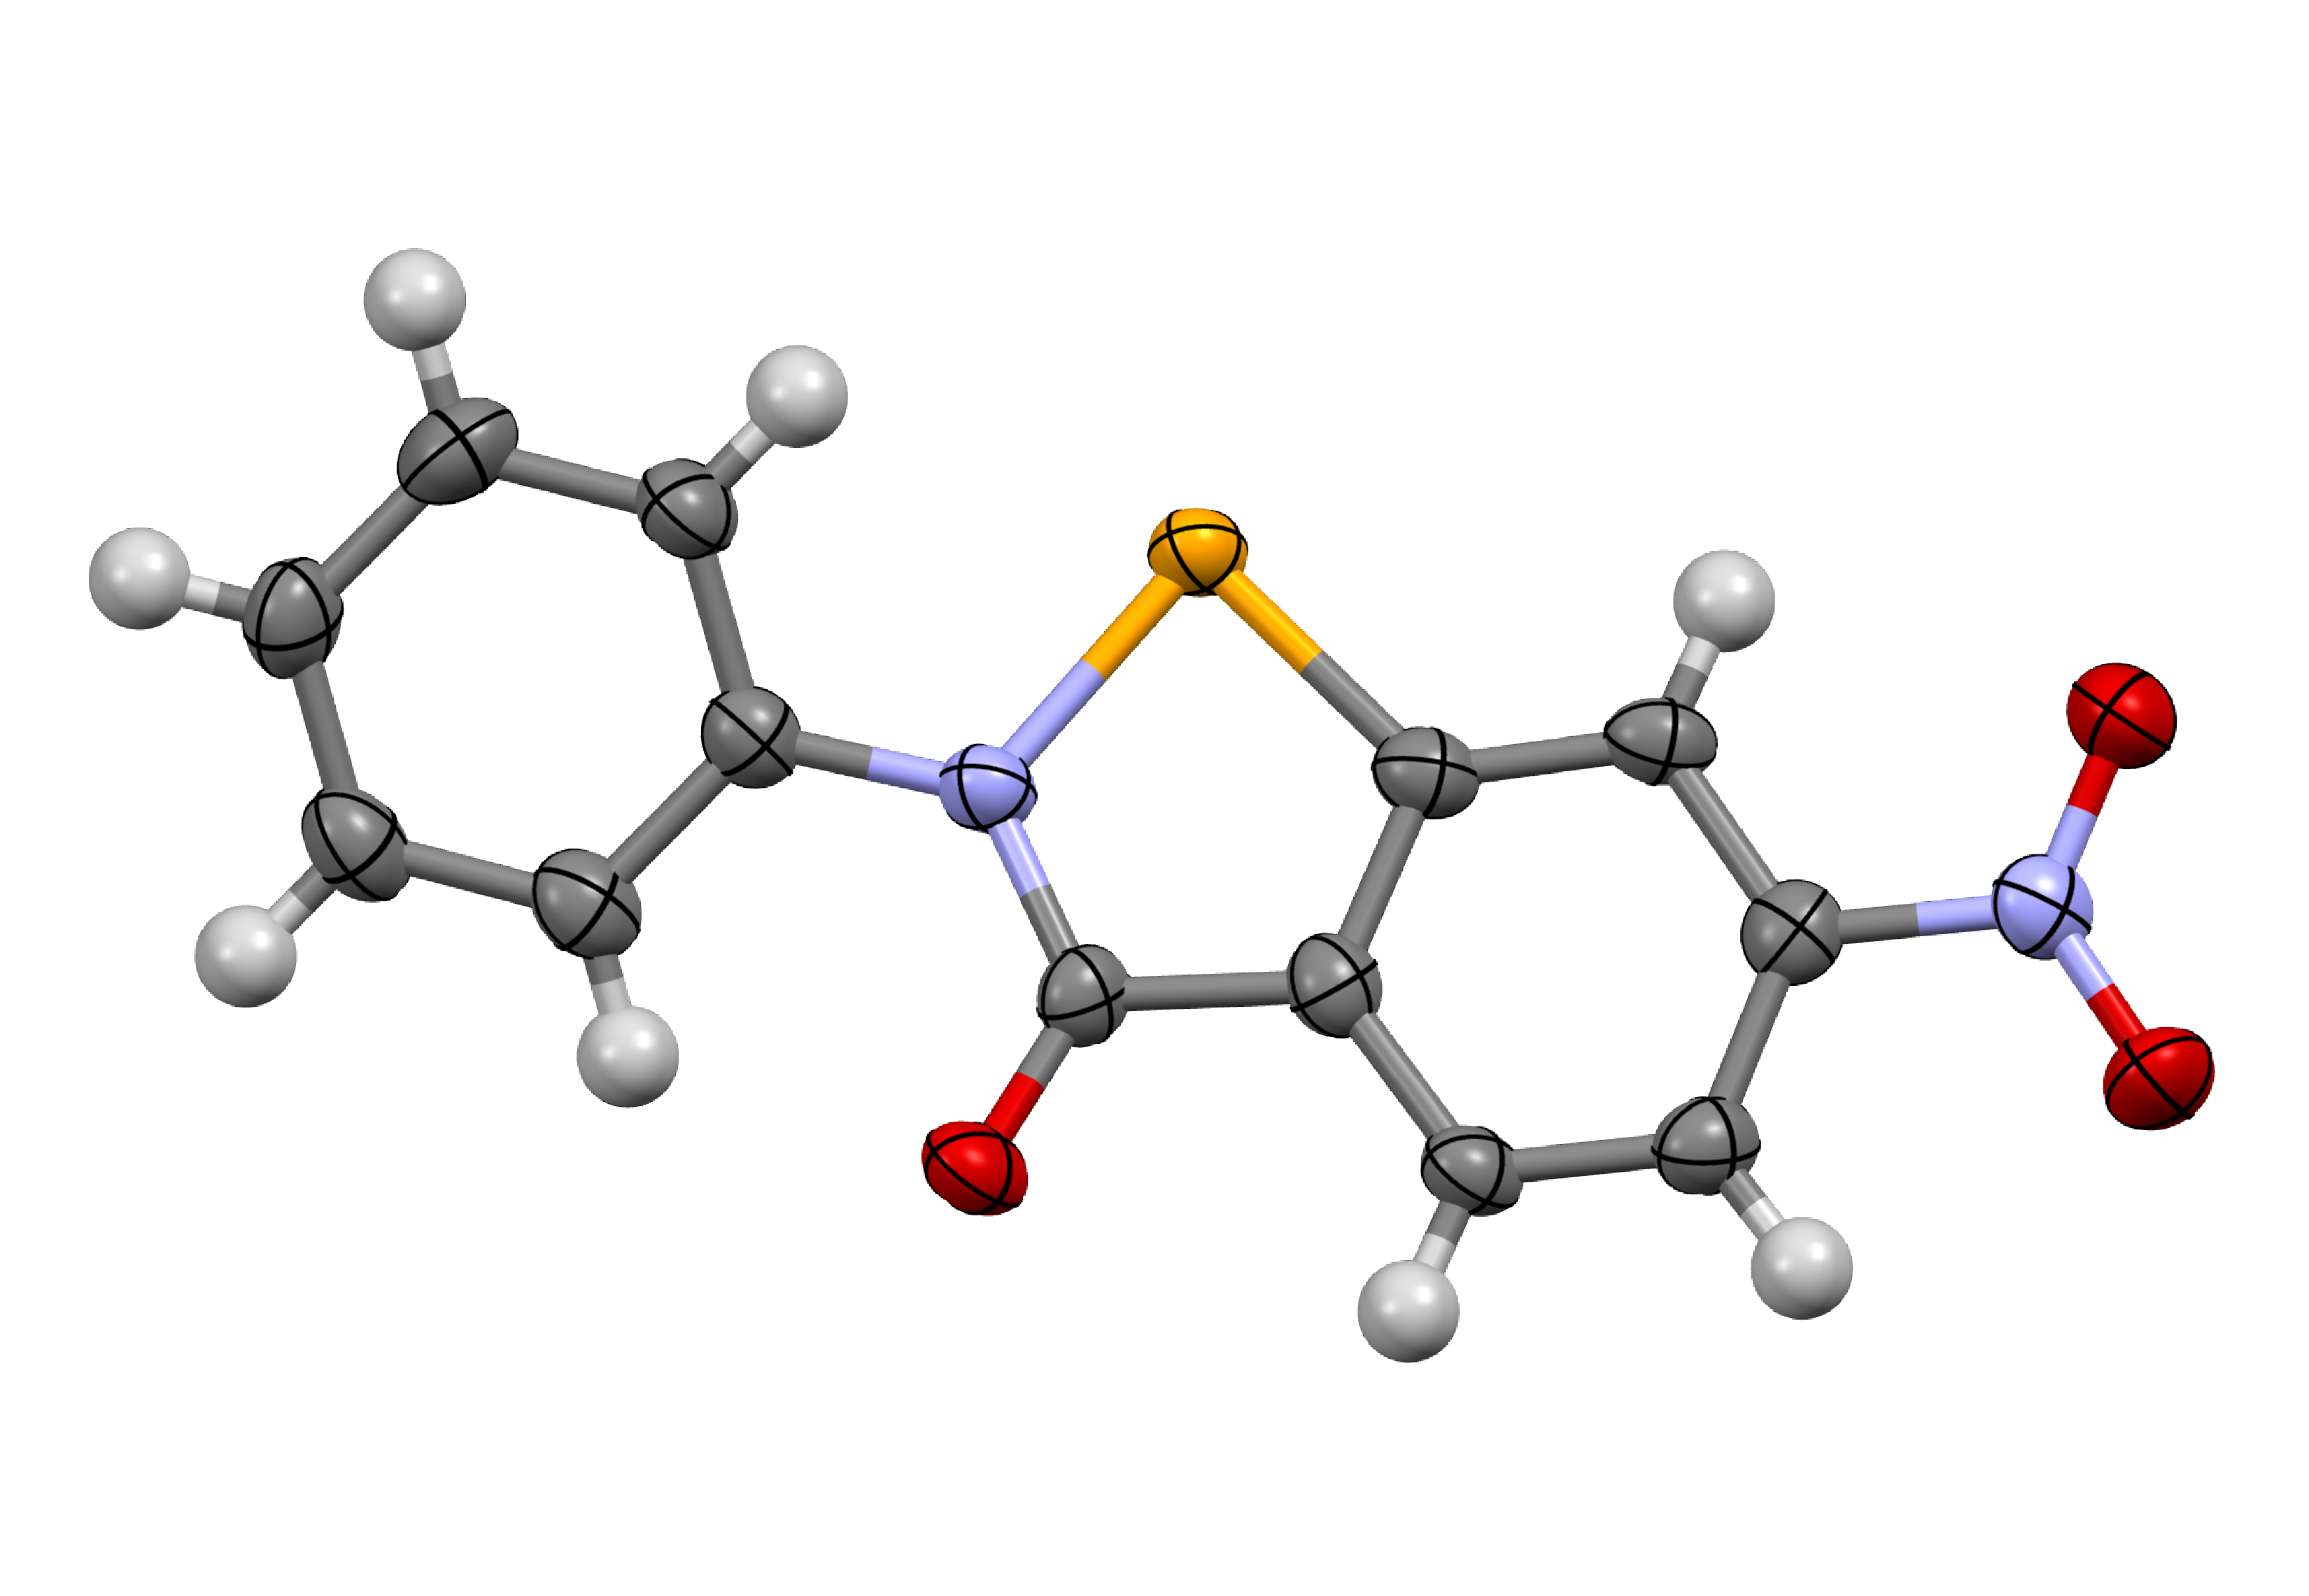
\includegraphics[width=0.8\linewidth]{Figures/ebs-3no2-xray.pdf}
    \caption{X-ray crystal structure of \refcmpd{ebs-3no2}.}
    \label{fig:ebs-3no2-xray}
\end{figure}

\subsubsection{Preparation of benzisoselenazolinone \refcmpd{ebs-h}}
Aqueous ammonia (30\%, 637~$\mu$L, 10~mmol) was dissolved in acetonitrile (5~mL), cooled to 0~\degree~C, and to this was added a solution of the selenyl chloride \cmpd{dichloride} (5~mmol) in a further 10~mL anhydrous acetonitrile.
The mixture was stirred at room temperature for 30~minutes, then the solvent evaporated \emph{in vacuo}, and the resulting solid washed with water (5~mL) to afford benzisoselenazolinone \cmpd{ebs-h} as an off white solid (858.4~mg, 87\%, m.p. XXX--XXX).

\footnotesize\paragraph{}

\ce{^{1}H} NMR (400~MHz, \ce{\emph{d}6}-DMSO) $\delta$ ppm
.

\ce{^{13}C} NMR (100~MHz, \ce{\emph{d}6}-DMSO) $\delta$ ppm
.

\ce{^{77}Se} NMR (0~MHz, \ce{\emph{d}6}-DMSO) $\delta$ ppm
.

MS (ESI +ve) m/z XXX (\ce{MH+}) \ce{XXXX+} requires XXXX ($\Delta$=0~ppm).

\normalsize


\subsubsection[Preparation of \refcmpd{ebs-3no2-4nh2}]{Preparation of 2-(4-amino-3-nitrophenyl)benzo[\emph{d}][1,2]selenazol-3(2\emph{H})-one \refcmpd{ebs-3no2-4nh2}}
Diselenide \cmpd{diselenide} (1.2025~g, 3.005~mmol) was dissolved in thionyl chloride (20~mL) and refluxed for 30~minutes, and the colour changed from purple to light yellow.
Excess thionyl chloride was removed \emph{in vacuo}, and the residue dissolved in anhydrous THF (50~mL).
To this was added a solution of 2-nitro-1,4-phenylenediamine (991.9~mg, 6.477~mmol) and triethylamine (3~mL, dist. from \ce{CaH2}) in anhydrous THF (50~mL).
This mixture was stirred at room temperature for 18~h, then filtered, washing the precipitate with water, to afford 2-(4-amino-3-nitrophenyl)benzo[\emph{d}][1,2]selenazol-3(2\emph{H})-one \cmpd{ebs-3no2-4nh2} as a brick red solid (940~mg, 61\%, m.p. (DMF) 300.8--302.0~\degree~C).

\footnotesize\paragraph{}

\ce{^{1}H} NMR (400~MHz, \ce{\emph{d}6}-DMSO) $\delta$ ppm
7.08 (d, \emph{J}=9.00~Hz, 1 H),
7.46 (t, \emph{J}=7.43~Hz, 1 H),
7.55 (s, 2 H),
7.59--7.70 (m, 2 H),
7.86 (d, \emph{J}=7.43~Hz, 1 H),
8.06 (d, \emph{J}=7.83~Hz, 1 H),
8.12 (d, \emph{J}=1.96~Hz, 1 H).

\ce{^{13}C} NMR (100~MHz, \ce{\emph{d}6}-DMSO) $\delta$ ppm
120.29 (s),
121.49 (s),
126.32 (s),
126.71 (s),
127.77 (s),
128.31 (s),
128.45 (s),
129.68 (s),
132.66 (s),
134.13 (s),
139.33 (s),
145.03 (s),
165.70 (s).

MS (ESI +ve) m/z 335.9882 (\ce{MH+}) \ce{C13H10N3O3Se+} requires 335.9881 ($\Delta$=0.298~ppm).

\normalsize


\subsubsection[Preparation of \refcmpd{ebs-3no2-4nh-2py}]{Preparation of \emph{N}-(2-nitro-4-(3-oxobenzo[\emph{d}][1,2]selenazol-2(3\emph{H})-yl)phenyl)picolinamide \refcmpd{ebs-3no2-4nh-2py}}
Picolinic acid (256.6~mg, 2.084~mmol) was dissolved in anhydrous THF (5~mL) and triethylamine (1~mL, dist. from \ce{CaH2}), then trichlorobenzoyl chloride (325~uL) was added and the mixture stirred for 10~minutes.
The nitroaniline \cmpd{ebs-3no2-4nh2} (242.8~mg, 0.956~mmol) was then added, and the mixture stirred under argon for 24~h, during which time the dark red colour faded to give a yellow solution.
The mixture was tipped into water (100~mL) and filtered to afford a yellow precipitate, which was recrystallised from pyridine (50~mL) to give 2-(4-amino-3-nitrophenyl)benzo[\emph{d}][1,2]selenazol-3(2\emph{H})-one \cmpd{ebs-3no2-4nh-2py} as a yellow solid (93.2~mg, 20\%, m.p. 342.7--343.7~\degree~C).

\footnotesize\paragraph{}

\ce{^{1}H} NMR (500~MHz, \ce{\emph{d}6}-DMSO) $\delta$ ppm
7.51 (t, \emph{J}=7.40~Hz, 1 H)
7.66--7.83 (m, 1 H)
7.94 (d, \emph{J}=7.63~Hz, 1 H)
8.04 (dd, \emph{J}=9.00, 2.40~Hz, 1 H)
8.09--8.17 (m, 2 H)
8.23 (d, \emph{J}=7.78~Hz, 1 H)
8.68 (d, \emph{J}=2.44~Hz, 1 H)
8.73 (d, \emph{J}=9.00~Hz, 1 H)
8.81 (d, \emph{J}=4.43~Hz, 1 H)
12.22 (s, 1 H)

MS (ESI +ve) m/z 441.0100 (\ce{MH+}) \ce{C19H13N4O4Se+} requires 441.0096 ($\Delta$=0.907~ppm).

\normalsize

\subsubsection{Preparation of 2-iodobenzoic anhydride \refcmpd{2-iodobenzoicanhydride}}
2-Iodobenzoic acid (1.9957~g, 8.045~mmol) and DCC (0.8457~g, 4.098~mmol) were stirred in anhydrous diethyl ether (10~mL) for 18~h. The white precipitate was filtered off, washing with cold anhydrous ether ($2\times$10~mL). The filtrate was concentrated \emph{in vacuo} to afford 2-iodobenzoic anhydride \cmpd{2-iodobenzoicanhydride} as an off-white solid (1.9623~g, 100\%).


\subsubsection{Preparation of \emph{N}-(3,4-dinitrophenyl)-2-iodobenzamide \refcmpd{iodoamide-3no2-4no2}}
A neat mixture 2-iodobenzoic anhydride \cmpd{2-iodobenzoicanhydride} (1.9226~g, 4.022~mmol), 3,4-dinitroaniline (0.7290~g, 3.981~mmol) and zinc iodide (0.2140~g, 0.673~mmol) was stirred at 80~\degree~C under an argon atmosphere. 
The melt was cooled to room temperature, dissolved in diethyl ether (40~mL), and the solution washed with 1~\textsc{M} \ce{HCl} (20~mL), 0.8~\textsc{M} sodium bicarbonate solution (50~mL), then brine (50~mL).
The organic phase was dried (\ce{MgSO4}), then evaporated to afford a yellow oil. 
This was triturated with petroleum ether (5~mL) with a few drops of dichloromethane to afford \emph{N}-(3,4-dinitrophenyl)-2-iodobenzamide \cmpd{iodoamide-3no2-4no2} as an off white solid (0.926~g, 56\%, m.p. XXX--XXX).\autocite{Shivani2007}

\footnotesize\paragraph{}

\ce{^{1}H} NMR (400~MHz, \ce{\emph{d}6}-DMSO) $\delta$ ppm
7.28 (td, \emph{J}=7.20, 1.96~Hz, 1 H),
7.48--7.61 (m, 2 H),
7.97 (d, \emph{J}=7.83~Hz, 1 H),
8.07 (dd, \emph{J}=8.80, 1.37~Hz, 1 H),
8.30 (d, \emph{J}=8.61~Hz, 1 H),
8.47 (d, \emph{J}=1.17~Hz, 1 H),
11.40 (s, 1 H).

\ce{^{13}C} NMR (100~MHz, \ce{\emph{d}6}-DMSO) $\delta$ ppm
93.91 (s),
115.06 (s),
122.90 (s),
127.96 (s),
128.72 (s),
128.76 (s),
132.28 (s),
136.30 (s),
139.69 (s),
142.03 (s),
144.21 (s),
144.76 (s),
168.92 (s).

MS (ESI +ve) m/z ??? (\ce{MH+}) \ce{C13H9IN3O5+} requires 413.9581 ($\Delta$=0~ppm).

\normalsize

\subsubsection{Preparation of 6-bromo-2-phenyl-1\textbf{H}-benzo[\emph{d}]imidazole}

\printbibliography[heading=subbibliography]
\end{refsection}